%%%%%%%%%%%%%%%%%%%%%%%%%%%%%%%%%%%%%%%%%
% Masters/Doctoral Thesis 
% LaTeX Template
% Version 2.5 (27/8/17)
%
% This template was downloaded from:
% http://www.LaTeXTemplates.com
%
% Version 2.x major modifications by:
% Vel (vel@latextemplates.com)
%
% This template is based on a template by:
% Steve Gunn (http://users.ecs.soton.ac.uk/srg/softwaretools/document/templates/)
% Sunil Patel (http://www.sunilpatel.co.uk/thesis-template/)
%
% Template license:
% CC BY-NC-SA 3.0 (http://creativecommons.org/licenses/by-nc-sa/3.0/)
%
%%%%%%%%%%%%%%%%%%%%%%%%%%%%%%%%%%%%%%%%%

%----------------------------------------------------------------------------------------
%	PACKAGES AND OTHER DOCUMENT CONFIGURATIONS
%----------------------------------------------------------------------------------------

\documentclass[
11pt, % The default document font size, options: 10pt, 11pt, 12pt
oneside, % Two side (alternating margins) for binding by default, uncomment to switch to one side
english, % ngerman for German
singlespacing, % Single line spacing, alternatives: onehalfspacing or doublespacing
%draft, % Uncomment to enable draft mode (no pictures, no links, overfull hboxes indicated)
%nolistspacing, % If the document is onehalfspacing or doublespacing, uncomment this to set spacing in lists to single
%liststotoc, % Uncomment to add the list of figures/tables/etc to the table of contents
%toctotoc, % Uncomment to add the main table of contents to the table of contents
%parskip, % Uncomment to add space between paragraphs
%nohyperref, % Uncomment to not load the hyperref package
headsepline, % Uncomment to get a line under the header
%chapterinoneline, % Uncomment to place the chapter title next to the number on one line
%consistentlayout, % Uncomment to change the layout of the declaration, abstract and acknowledgements pages to match the default layout
]{MastersDoctoralThesis} % The class file specifying the document structure

\usepackage[utf8]{inputenc} % Required for inputting international characters
\usepackage[T1]{fontenc} % Output font encoding for international characters
\usepackage{amsmath}
\usepackage{amsfonts}
\usepackage{amssymb}

\usepackage{mathpazo} % Use the Palatino font by default

\usepackage[backend=bibtex,style=authoryear,natbib=true]{biblatex} % Use the bibtex backend with the authoryear citation style (which resembles APA)

\addbibresource{example.bib} % The filename of the bibliography

\usepackage[autostyle=true]{csquotes} % Required to generate language-dependent quotes in the bibliography

%----------------------------------------------------------------------------------------
%	MARGIN SETTINGS
%----------------------------------------------------------------------------------------

\geometry{
	paper=a4paper, % Change to letterpaper for US letter
	inner=2.5cm, % Inner margin
	outer=3.8cm, % Outer margin
	bindingoffset=.5cm, % Binding offset
	top=1.5cm, % Top margin
	bottom=1.5cm, % Bottom margin
	%showframe, % Uncomment to show how the type block is set on the page
}

%----------------------------------------------------------------------------------------
%	THESIS INFORMATION
%----------------------------------------------------------------------------------------

\thesistitle{Reconstructing locomotion in VR from WIP (Walking-In-Place) motion : an IMU-based, inside-out approach} % Your thesis title, this is used in the title and abstract, print it elsewhere with \ttitle
\supervisor{Prof. Frank C. \textsc{Park}} % Your supervisor's name, this is used in the title page, print it elsewhere with \supname
\examiner{} % Your examiner's name, this is not currently used anywhere in the template, print it elsewhere with \examname
\degree{Bachelor of Engineering} % Your degree name, this is used in the title page and abstract, print it elsewhere with \degreename
\author{JiGang \textsc{Kim}} % Your name, this is used in the title page and abstract, print it elsewhere with \authorname
\addresses{} % Your address, this is not currently used anywhere in the template, print it elsewhere with \addressname

\subject{Robotics} % Your subject area, this is not currently used anywhere in the template, print it elsewhere with \subjectname
\keywords{} % Keywords for your thesis, this is not currently used anywhere in the template, print it elsewhere with \keywordnames
\university{\href{https://snu.ac.kr}{Seoul National University}} % Your university's name and URL, this is used in the title page and abstract, print it elsewhere with \univname
\department{\href{http://mae.snu.ac.kr}{Department of Mechanical \& Aerospace Engineering}} % Your department's name and URL, this is used in the title page and abstract, print it elsewhere with \deptname
\group{\href{http://robotics.snu.ac.kr/fcp}{Robotics Laboratory}} % Your research group's name and URL, this is used in the title page, print it elsewhere with \groupname
\faculty{} % Your faculty's name and URL, this is used in the title page and abstract, print it elsewhere with \facname

\AtBeginDocument{
\hypersetup{pdftitle=\ttitle} % Set the PDF's title to your title
\hypersetup{pdfauthor=\authorname} % Set the PDF's author to your name
\hypersetup{pdfkeywords=\keywordnames} % Set the PDF's keywords to your keywords
}

\begin{document}

\frontmatter % Use roman page numbering style (i, ii, iii, iv...) for the pre-content pages

\pagestyle{plain} % Default to the plain heading style until the thesis style is called for the body content

%----------------------------------------------------------------------------------------
%	TITLE PAGE
%----------------------------------------------------------------------------------------

\begin{titlepage}
\begin{center}

\vspace*{.06\textheight}
{\scshape\LARGE \univname\par}\vspace{1.5cm} % University name
\textsc{\Large Bachelor Thesis}\\[0.5cm] % Thesis type

\HRule \\[0.4cm] % Horizontal line
{\huge \bfseries \ttitle\par}\vspace{0.4cm} % Thesis title
\HRule \\[1.5cm] % Horizontal line
 
\begin{minipage}[t]{0.4\textwidth}
\begin{flushleft} \large
\emph{Author:}\\
\authorname % Author name - remove the \href bracket to remove the link
\end{flushleft}
\end{minipage}
\begin{minipage}[t]{0.4\textwidth}
\begin{flushright} \large
\emph{Supervisor:} \\
\supname % Supervisor name - remove the \href bracket to remove the link  
\end{flushright}
\end{minipage}\\[3cm]
 
\vfill

\large \textit{A thesis submitted in fulfillment of the requirements\\ for the degree of \degreename}\\[0.3cm] % University requirement text
\textit{in the}\\[0.4cm]
\groupname\\\deptname\\[2cm] % Research group name and department name
 
\vfill

{\large \today}\\[4cm] % Date
%\includegraphics{Logo} % University/department logo - uncomment to place it
 
\vfill
\end{center}
\end{titlepage}

%----------------------------------------------------------------------------------------
%	DECLARATION PAGE
%----------------------------------------------------------------------------------------

\begin{declaration}
\addchaptertocentry{\authorshipname} % Add the declaration to the table of contents
\noindent I, \authorname, declare that this thesis titled, \enquote{\ttitle} and the work presented in it are my own. I confirm that:

\begin{itemize} 
\item This work was done wholly or mainly while in candidature for a research degree at this University.
\item Where any part of this thesis has previously been submitted for a degree or any other qualification at this University or any other institution, this has been clearly stated.
\item Where I have consulted the published work of others, this is always clearly attributed.
\item Where I have quoted from the work of others, the source is always given. With the exception of such quotations, this thesis is entirely my own work.
\item I have acknowledged all main sources of help.
\item Where the thesis is based on work done by myself jointly with others, I have made clear exactly what was done by others and what I have contributed myself.\\
\end{itemize}
 
\noindent Signed:\\
\rule[0.5em]{25em}{0.5pt} % This prints a line for the signature
 
\noindent Date:\\
\rule[0.5em]{25em}{0.5pt} % This prints a line to write the date
\end{declaration}

\cleardoublepage

%----------------------------------------------------------------------------------------
%	QUOTATION PAGE
%----------------------------------------------------------------------------------------

%\vspace*{0.2\textheight}
%
%\noindent\enquote{\itshape Thanks to my solid academic training, today I can write hundreds of words on virtually any topic without possessing a shred of information, which is how I got a good job in journalism.}\bigbreak
%
%\hfill Dave Barry

%----------------------------------------------------------------------------------------
%	ABSTRACT PAGE
%----------------------------------------------------------------------------------------

\begin{abstract}
\addchaptertocentry{\abstractname} % Add the abstract to the table of contents
WIP (Walking-In-Place) motion based VR (Virtual Reality) locomotion techniques simulate horizontal motion in virtual environments from vertical foot motion. Due to its similarity to real walking, WIP provides intuitive and immersive user interface for navigating vast virtual environments within the confines of limited physical space. Numerous past literatures on this topic implemented costly and complex systems to demonstrate their algorithms. The proposed approach requires a simple setup of two IMU (Inertial Measurement Unit) sensor modules attached to each foot and a Android phone capable of running Google Cardboard. With the proposed setup it is possible to track WIP motion as well as walking motion. This has been possible by incorporating key ideas from PDR (Pedestrian Dead Reckoning) algorithms, which aim to accurately track the position of a pedestrian without receiving any information from external sources. This paper presents a low-cost, natural interface for navigating VEs by synthesizing a personalized locomotion from WIP motion with offline gait analysis.
\\\\KEYWORDS: Walking-In-Place (WIP), Inside-Out, Virtual Reality (VR), Virtual Environment (VE), Virtual Locomotion, Inertial Measurement Unit (IMU)
\end{abstract}

%----------------------------------------------------------------------------------------
%	ACKNOWLEDGEMENTS
%----------------------------------------------------------------------------------------

\begin{acknowledgements}
\addchaptertocentry{\acknowledgementname} % Add the acknowledgements to the table of contents
This research has been funded by Korea Institute of Science and Technology (KIST). Special thanks to Dr. Kim and Dr. Moon for their advice and assistance and Mr. Jeong for providing source code and assets for Unity client and TCP server.
\end{acknowledgements}

%----------------------------------------------------------------------------------------
%	LIST OF CONTENTS/FIGURES/TABLES PAGES
%----------------------------------------------------------------------------------------

\tableofcontents % Prints the main table of contents

\listoffigures % Prints the list of figures

%\listoftables % Prints the list of tables

%----------------------------------------------------------------------------------------
%	ABBREVIATIONS
%----------------------------------------------------------------------------------------

%\begin{abbreviations}{ll} % Include a list of abbreviations (a table of two columns)
%
%\textbf{LAH} & \textbf{L}ist \textbf{A}bbreviations \textbf{H}ere\\
%\textbf{WSF} & \textbf{W}hat (it) \textbf{S}tands \textbf{F}or\\
%
%\end{abbreviations}

%----------------------------------------------------------------------------------------
%	PHYSICAL CONSTANTS/OTHER DEFINITIONS
%----------------------------------------------------------------------------------------

%\begin{constants}{lr@{${}={}$}l} % The list of physical constants is a three column table
%
%% The \SI{}{} command is provided by the siunitx package, see its documentation for instructions on how to use it
%
%Gravitational Acceleration & $g_{0}$ & \SI{9.81}{\meter\per\second^{2}} \\
%%Constant Name & $Symbol$ & $Constant Value$ with units\\
%
%\end{constants}

%----------------------------------------------------------------------------------------
%	SYMBOLS
%----------------------------------------------------------------------------------------

%\begin{symbols}{lll} % Include a list of Symbols (a three column table)
%
%$a$ & distance & \si{\meter} \\
%$P$ & power & \si{\watt} (\si{\joule\per\second}) \\
%%Symbol & Name & Unit \\
%
%\addlinespace % Gap to separate the Roman symbols from the Greek
%
%$\omega$ & angular frequency & \si{\radian} \\
%
%\end{symbols}

%----------------------------------------------------------------------------------------
%	DEDICATION
%----------------------------------------------------------------------------------------

%\dedicatory{For/Dedicated to/To my\ldots} 

%----------------------------------------------------------------------------------------
%	THESIS CONTENT - CHAPTERS
%----------------------------------------------------------------------------------------

\mainmatter % Begin numeric (1,2,3...) page numbering

\pagestyle{thesis} % Return the page headers back to the "thesis" style

% Include the chapters of the thesis as separate files from the Chapters folder
% Uncomment the lines as you write the chapters

%% Chapter 1

\chapter{Introduction} % Main chapter title

\label{Chapter100} % For referencing the chapter elsewhere, use \ref{Chapter1} 

%----------------------------------------------------------------------------------------

% Define some commands to keep the formatting separated from the content 
\newcommand{\keyword}[1]{\textbf{#1}}
\newcommand{\tabhead}[1]{\textbf{#1}}
\newcommand{\code}[1]{\texttt{#1}}
\newcommand{\file}[1]{\texttt{\bfseries#1}}
\newcommand{\option}[1]{\texttt{\itshape#1}}

%----------------------------------------------------------------------------------------

\section{Welcome and Thank You}
Welcome to this \LaTeX{} Thesis Template, a beautiful and easy to use template for writing a thesis using the \LaTeX{} typesetting system.

If you are writing a thesis (or will be in the future) and its subject is technical or mathematical (though it doesn't have to be), then creating it in \LaTeX{} is highly recommended as a way to make sure you can just get down to the essential writing without having to worry over formatting or wasting time arguing with your word processor.

\LaTeX{} is easily able to professionally typeset documents that run to hundreds or thousands of pages long. With simple mark-up commands, it automatically sets out the table of contents, margins, page headers and footers and keeps the formatting consistent and beautiful. One of its main strengths is the way it can easily typeset mathematics, even \emph{heavy} mathematics. Even if those equations are the most horribly twisted and most difficult mathematical problems that can only be solved on a super-computer, you can at least count on \LaTeX{} to make them look stunning.

%----------------------------------------------------------------------------------------

\section{Learning \LaTeX{}}

\LaTeX{} is not a \textsc{wysiwyg} (What You See is What You Get) program, unlike word processors such as Microsoft Word or Apple's Pages. Instead, a document written for \LaTeX{} is actually a simple, plain text file that contains \emph{no formatting}. You tell \LaTeX{} how you want the formatting in the finished document by writing in simple commands amongst the text, for example, if I want to use \emph{italic text for emphasis}, I write the \verb|\emph{text}| command and put the text I want in italics in between the curly braces. This means that \LaTeX{} is a \enquote{mark-up} language, very much like HTML.

\subsection{A (not so short) Introduction to \LaTeX{}}

If you are new to \LaTeX{}, there is a very good eBook -- freely available online as a PDF file -- called, \enquote{The Not So Short Introduction to \LaTeX{}}. The book's title is typically shortened to just \emph{lshort}. You can download the latest version (as it is occasionally updated) from here:
\url{http://www.ctan.org/tex-archive/info/lshort/english/lshort.pdf}

It is also available in several other languages. Find yours from the list on this page: \url{http://www.ctan.org/tex-archive/info/lshort/}

It is recommended to take a little time out to learn how to use \LaTeX{} by creating several, small `test' documents, or having a close look at several templates on:\\ 
\url{http://www.LaTeXTemplates.com}\\ 
Making the effort now means you're not stuck learning the system when what you \emph{really} need to be doing is writing your thesis.

\subsection{A Short Math Guide for \LaTeX{}}

If you are writing a technical or mathematical thesis, then you may want to read the document by the AMS (American Mathematical Society) called, \enquote{A Short Math Guide for \LaTeX{}}. It can be found online here:
\url{http://www.ams.org/tex/amslatex.html}
under the \enquote{Additional Documentation} section towards the bottom of the page.

\subsection{Common \LaTeX{} Math Symbols}
There are a multitude of mathematical symbols available for \LaTeX{} and it would take a great effort to learn the commands for them all. The most common ones you are likely to use are shown on this page:
\url{http://www.sunilpatel.co.uk/latex-type/latex-math-symbols/}

You can use this page as a reference or crib sheet, the symbols are rendered as large, high quality images so you can quickly find the \LaTeX{} command for the symbol you need.

\subsection{\LaTeX{} on a Mac}
 
The \LaTeX{} distribution is available for many systems including Windows, Linux and Mac OS X. The package for OS X is called MacTeX and it contains all the applications you need -- bundled together and pre-customized -- for a fully working \LaTeX{} environment and work flow.
 
MacTeX includes a custom dedicated \LaTeX{} editor called TeXShop for writing your `\file{.tex}' files and BibDesk: a program to manage your references and create your bibliography section just as easily as managing songs and creating playlists in iTunes.

%----------------------------------------------------------------------------------------

\section{Getting Started with this Template}

If you are familiar with \LaTeX{}, then you should explore the directory structure of the template and then proceed to place your own information into the \emph{THESIS INFORMATION} block of the \file{main.tex} file. You can then modify the rest of this file to your unique specifications based on your degree/university. Section \ref{FillingFile} on page \pageref{FillingFile} will help you do this. Make sure you also read section \ref{ThesisConventions} about thesis conventions to get the most out of this template.

If you are new to \LaTeX{} it is recommended that you carry on reading through the rest of the information in this document.

Before you begin using this template you should ensure that its style complies with the thesis style guidelines imposed by your institution. In most cases this template style and layout will be suitable. If it is not, it may only require a small change to bring the template in line with your institution's recommendations. These modifications will need to be done on the \file{MastersDoctoralThesis.cls} file.

\subsection{About this Template}

This \LaTeX{} Thesis Template is originally based and created around a \LaTeX{} style file created by Steve R.\ Gunn from the University of Southampton (UK), department of Electronics and Computer Science. You can find his original thesis style file at his site, here:
\url{http://www.ecs.soton.ac.uk/~srg/softwaretools/document/templates/}

Steve's \file{ecsthesis.cls} was then taken by Sunil Patel who modified it by creating a skeleton framework and folder structure to place the thesis files in. The resulting template can be found on Sunil's site here:
\url{http://www.sunilpatel.co.uk/thesis-template}

Sunil's template was made available through \url{http://www.LaTeXTemplates.com} where it was modified many times based on user requests and questions. Version 2.0 and onwards of this template represents a major modification to Sunil's template and is, in fact, hardly recognisable. The work to make version 2.0 possible was carried out by \href{mailto:vel@latextemplates.com}{Vel} and Johannes Böttcher.

%----------------------------------------------------------------------------------------

\section{What this Template Includes}

\subsection{Folders}

This template comes as a single zip file that expands out to several files and folders. The folder names are mostly self-explanatory:

\keyword{Appendices} -- this is the folder where you put the appendices. Each appendix should go into its own separate \file{.tex} file. An example and template are included in the directory.

\keyword{Chapters} -- this is the folder where you put the thesis chapters. A thesis usually has about six chapters, though there is no hard rule on this. Each chapter should go in its own separate \file{.tex} file and they can be split as:
\begin{itemize}
\item Chapter 1: Introduction to the thesis topic
\item Chapter 2: Background information and theory
\item Chapter 3: (Laboratory) experimental setup
\item Chapter 4: Details of experiment 1
\item Chapter 5: Details of experiment 2
\item Chapter 6: Discussion of the experimental results
\item Chapter 7: Conclusion and future directions
\end{itemize}
This chapter layout is specialised for the experimental sciences, your discipline may be different.

\keyword{Figures} -- this folder contains all figures for the thesis. These are the final images that will go into the thesis document.

\subsection{Files}

Included are also several files, most of them are plain text and you can see their contents in a text editor. After initial compilation, you will see that more auxiliary files are created by \LaTeX{} or BibTeX and which you don't need to delete or worry about:

\keyword{example.bib} -- this is an important file that contains all the bibliographic information and references that you will be citing in the thesis for use with BibTeX. You can write it manually, but there are reference manager programs available that will create and manage it for you. Bibliographies in \LaTeX{} are a large subject and you may need to read about BibTeX before starting with this. Many modern reference managers will allow you to export your references in BibTeX format which greatly eases the amount of work you have to do.

\keyword{MastersDoctoralThesis.cls} -- this is an important file. It is the class file that tells \LaTeX{} how to format the thesis. 

\keyword{main.pdf} -- this is your beautifully typeset thesis (in the PDF file format) created by \LaTeX{}. It is supplied in the PDF with the template and after you compile the template you should get an identical version.

\keyword{main.tex} -- this is an important file. This is the file that you tell \LaTeX{} to compile to produce your thesis as a PDF file. It contains the framework and constructs that tell \LaTeX{} how to layout the thesis. It is heavily commented so you can read exactly what each line of code does and why it is there. After you put your own information into the \emph{THESIS INFORMATION} block -- you have now started your thesis!

Files that are \emph{not} included, but are created by \LaTeX{} as auxiliary files include:

\keyword{main.aux} -- this is an auxiliary file generated by \LaTeX{}, if it is deleted \LaTeX{} simply regenerates it when you run the main \file{.tex} file.

\keyword{main.bbl} -- this is an auxiliary file generated by BibTeX, if it is deleted, BibTeX simply regenerates it when you run the \file{main.aux} file. Whereas the \file{.bib} file contains all the references you have, this \file{.bbl} file contains the references you have actually cited in the thesis and is used to build the bibliography section of the thesis.

\keyword{main.blg} -- this is an auxiliary file generated by BibTeX, if it is deleted BibTeX simply regenerates it when you run the main \file{.aux} file.

\keyword{main.lof} -- this is an auxiliary file generated by \LaTeX{}, if it is deleted \LaTeX{} simply regenerates it when you run the main \file{.tex} file. It tells \LaTeX{} how to build the \emph{List of Figures} section.

\keyword{main.log} -- this is an auxiliary file generated by \LaTeX{}, if it is deleted \LaTeX{} simply regenerates it when you run the main \file{.tex} file. It contains messages from \LaTeX{}, if you receive errors and warnings from \LaTeX{}, they will be in this \file{.log} file.

\keyword{main.lot} -- this is an auxiliary file generated by \LaTeX{}, if it is deleted \LaTeX{} simply regenerates it when you run the main \file{.tex} file. It tells \LaTeX{} how to build the \emph{List of Tables} section.

\keyword{main.out} -- this is an auxiliary file generated by \LaTeX{}, if it is deleted \LaTeX{} simply regenerates it when you run the main \file{.tex} file.

So from this long list, only the files with the \file{.bib}, \file{.cls} and \file{.tex} extensions are the most important ones. The other auxiliary files can be ignored or deleted as \LaTeX{} and BibTeX will regenerate them.

%----------------------------------------------------------------------------------------

\section{Filling in Your Information in the \file{main.tex} File}\label{FillingFile}

You will need to personalise the thesis template and make it your own by filling in your own information. This is done by editing the \file{main.tex} file in a text editor or your favourite LaTeX environment.

Open the file and scroll down to the third large block titled \emph{THESIS INFORMATION} where you can see the entries for \emph{University Name}, \emph{Department Name}, etc \ldots

Fill out the information about yourself, your group and institution. You can also insert web links, if you do, make sure you use the full URL, including the \code{http://} for this. If you don't want these to be linked, simply remove the \verb|\href{url}{name}| and only leave the name.

When you have done this, save the file and recompile \code{main.tex}. All the information you filled in should now be in the PDF, complete with web links. You can now begin your thesis proper!

%----------------------------------------------------------------------------------------

\section{The \code{main.tex} File Explained}

The \file{main.tex} file contains the structure of the thesis. There are plenty of written comments that explain what pages, sections and formatting the \LaTeX{} code is creating. Each major document element is divided into commented blocks with titles in all capitals to make it obvious what the following bit of code is doing. Initially there seems to be a lot of \LaTeX{} code, but this is all formatting, and it has all been taken care of so you don't have to do it.

Begin by checking that your information on the title page is correct. For the thesis declaration, your institution may insist on something different than the text given. If this is the case, just replace what you see with what is required in the \emph{DECLARATION PAGE} block.

Then comes a page which contains a funny quote. You can put your own, or quote your favourite scientist, author, person, and so on. Make sure to put the name of the person who you took the quote from.

Following this is the abstract page which summarises your work in a condensed way and can almost be used as a standalone document to describe what you have done. The text you write will cause the heading to move up so don't worry about running out of space.

Next come the acknowledgements. On this page, write about all the people who you wish to thank (not forgetting parents, partners and your advisor/supervisor).

The contents pages, list of figures and tables are all taken care of for you and do not need to be manually created or edited. The next set of pages are more likely to be optional and can be deleted since they are for a more technical thesis: insert a list of abbreviations you have used in the thesis, then a list of the physical constants and numbers you refer to and finally, a list of mathematical symbols used in any formulae. Making the effort to fill these tables means the reader has a one-stop place to refer to instead of searching the internet and references to try and find out what you meant by certain abbreviations or symbols.

The list of symbols is split into the Roman and Greek alphabets. Whereas the abbreviations and symbols ought to be listed in alphabetical order (and this is \emph{not} done automatically for you) the list of physical constants should be grouped into similar themes.

The next page contains a one line dedication. Who will you dedicate your thesis to?

Finally, there is the block where the chapters are included. Uncomment the lines (delete the \code{\%} character) as you write the chapters. Each chapter should be written in its own file and put into the \emph{Chapters} folder and named \file{Chapter1}, \file{Chapter2}, etc\ldots Similarly for the appendices, uncomment the lines as you need them. Each appendix should go into its own file and placed in the \emph{Appendices} folder.

After the preamble, chapters and appendices finally comes the bibliography. The bibliography style (called \option{authoryear}) is used for the bibliography and is a fully featured style that will even include links to where the referenced paper can be found online. Do not underestimate how grateful your reader will be to find that a reference to a paper is just a click away. Of course, this relies on you putting the URL information into the BibTeX file in the first place.

%----------------------------------------------------------------------------------------

\section{Thesis Features and Conventions}\label{ThesisConventions}

To get the best out of this template, there are a few conventions that you may want to follow.

One of the most important (and most difficult) things to keep track of in such a long document as a thesis is consistency. Using certain conventions and ways of doing things (such as using a Todo list) makes the job easier. Of course, all of these are optional and you can adopt your own method.

\subsection{Printing Format}

This thesis template is designed for double sided printing (i.e. content on the front and back of pages) as most theses are printed and bound this way. Switching to one sided printing is as simple as uncommenting the \option{oneside} option of the \code{documentclass} command at the top of the \file{main.tex} file. You may then wish to adjust the margins to suit specifications from your institution.

The headers for the pages contain the page number on the outer side (so it is easy to flick through to the page you want) and the chapter name on the inner side.

The text is set to 11 point by default with single line spacing, again, you can tune the text size and spacing should you want or need to using the options at the very start of \file{main.tex}. The spacing can be changed similarly by replacing the \option{singlespacing} with \option{onehalfspacing} or \option{doublespacing}.

\subsection{Using US Letter Paper}

The paper size used in the template is A4, which is the standard size in Europe. If you are using this thesis template elsewhere and particularly in the United States, then you may have to change the A4 paper size to the US Letter size. This can be done in the margins settings section in \file{main.tex}.

Due to the differences in the paper size, the resulting margins may be different to what you like or require (as it is common for institutions to dictate certain margin sizes). If this is the case, then the margin sizes can be tweaked by modifying the values in the same block as where you set the paper size. Now your document should be set up for US Letter paper size with suitable margins.

\subsection{References}

The \code{biblatex} package is used to format the bibliography and inserts references such as this one \parencite{Reference1}. The options used in the \file{main.tex} file mean that the in-text citations of references are formatted with the author(s) listed with the date of the publication. Multiple references are separated by semicolons (e.g. \parencite{Reference2, Reference1}) and references with more than three authors only show the first author with \emph{et al.} indicating there are more authors (e.g. \parencite{Reference3}). This is done automatically for you. To see how you use references, have a look at the \file{Chapter1.tex} source file. Many reference managers allow you to simply drag the reference into the document as you type.

Scientific references should come \emph{before} the punctuation mark if there is one (such as a comma or period). The same goes for footnotes\footnote{Such as this footnote, here down at the bottom of the page.}. You can change this but the most important thing is to keep the convention consistent throughout the thesis. Footnotes themselves should be full, descriptive sentences (beginning with a capital letter and ending with a full stop). The APA6 states: \enquote{Footnote numbers should be superscripted, [...], following any punctuation mark except a dash.} The Chicago manual of style states: \enquote{A note number should be placed at the end of a sentence or clause. The number follows any punctuation mark except the dash, which it precedes. It follows a closing parenthesis.}

The bibliography is typeset with references listed in alphabetical order by the first author's last name. This is similar to the APA referencing style. To see how \LaTeX{} typesets the bibliography, have a look at the very end of this document (or just click on the reference number links in in-text citations).

\subsubsection{A Note on bibtex}

The bibtex backend used in the template by default does not correctly handle unicode character encoding (i.e. "international" characters). You may see a warning about this in the compilation log and, if your references contain unicode characters, they may not show up correctly or at all. The solution to this is to use the biber backend instead of the outdated bibtex backend. This is done by finding this in \file{main.tex}: \option{backend=bibtex} and changing it to \option{backend=biber}. You will then need to delete all auxiliary BibTeX files and navigate to the template directory in your terminal (command prompt). Once there, simply type \code{biber main} and biber will compile your bibliography. You can then compile \file{main.tex} as normal and your bibliography will be updated. An alternative is to set up your LaTeX editor to compile with biber instead of bibtex, see \href{http://tex.stackexchange.com/questions/154751/biblatex-with-biber-configuring-my-editor-to-avoid-undefined-citations/}{here} for how to do this for various editors.

\subsection{Tables}

Tables are an important way of displaying your results, below is an example table which was generated with this code:

{\small
\begin{verbatim}
\begin{table}
\caption{The effects of treatments X and Y on the four groups studied.}
\label{tab:treatments}
\centering
\begin{tabular}{l l l}
\toprule
\tabhead{Groups} & \tabhead{Treatment X} & \tabhead{Treatment Y} \\
\midrule
1 & 0.2 & 0.8\\
2 & 0.17 & 0.7\\
3 & 0.24 & 0.75\\
4 & 0.68 & 0.3\\
\bottomrule\\
\end{tabular}
\end{table}
\end{verbatim}
}

\begin{table}
\caption{The effects of treatments X and Y on the four groups studied.}
\label{tab:treatments}
\centering
\begin{tabular}{l l l}
\toprule
\tabhead{Groups} & \tabhead{Treatment X} & \tabhead{Treatment Y} \\
\midrule
1 & 0.2 & 0.8\\
2 & 0.17 & 0.7\\
3 & 0.24 & 0.75\\
4 & 0.68 & 0.3\\
\bottomrule\\
\end{tabular}
\end{table}

You can reference tables with \verb|\ref{<label>}| where the label is defined within the table environment. See \file{Chapter1.tex} for an example of the label and citation (e.g. Table~\ref{tab:treatments}).

\subsection{Figures}

There will hopefully be many figures in your thesis (that should be placed in the \emph{Figures} folder). The way to insert figures into your thesis is to use a code template like this:
\begin{verbatim}
\begin{figure}
\centering

\includegraphics{Figures/Electron}
\decoRule
\caption[An Electron]{An electron (artist's impression).}
\label{fig:Electron}
\end{figure}
\end{verbatim}
Also look in the source file. Putting this code into the source file produces the picture of the electron that you can see in the figure below.

\begin{figure}[th]
\centering

\includegraphics{Figures/Electron}
\decoRule
\caption[An Electron]{An electron (artist's impression).}
\label{fig:Electron}
\end{figure}

Sometimes figures don't always appear where you write them in the source. The placement depends on how much space there is on the page for the figure. Sometimes there is not enough room to fit a figure directly where it should go (in relation to the text) and so \LaTeX{} puts it at the top of the next page. Positioning figures is the job of \LaTeX{} and so you should only worry about making them look good!

Figures usually should have captions just in case you need to refer to them (such as in Figure~\ref{fig:Electron}). The \verb|\caption| command contains two parts, the first part, inside the square brackets is the title that will appear in the \emph{List of Figures}, and so should be short. The second part in the curly brackets should contain the longer and more descriptive caption text.

The \verb|\decoRule| command is optional and simply puts an aesthetic horizontal line below the image. If you do this for one image, do it for all of them.

\LaTeX{} is capable of using images in pdf, jpg and png format.

\subsection{Typesetting mathematics}

If your thesis is going to contain heavy mathematical content, be sure that \LaTeX{} will make it look beautiful, even though it won't be able to solve the equations for you.

The \enquote{Not So Short Introduction to \LaTeX} (available on \href{http://www.ctan.org/tex-archive/info/lshort/english/lshort.pdf}{CTAN}) should tell you everything you need to know for most cases of typesetting mathematics. If you need more information, a much more thorough mathematical guide is available from the AMS called, \enquote{A Short Math Guide to \LaTeX} and can be downloaded from:
\url{ftp://ftp.ams.org/pub/tex/doc/amsmath/short-math-guide.pdf}

There are many different \LaTeX{} symbols to remember, luckily you can find the most common symbols in \href{http://ctan.org/pkg/comprehensive}{The Comprehensive \LaTeX~Symbol List}.

You can write an equation, which is automatically given an equation number by \LaTeX{} like this:
\begin{verbatim}
\begin{equation}
E = mc^{2}
\label{eqn:Einstein}
\end{equation}
\end{verbatim}

This will produce Einstein's famous energy-matter equivalence equation:
\begin{equation}
E = mc^{2}
\label{eqn:Einstein}
\end{equation}

All equations you write (which are not in the middle of paragraph text) are automatically given equation numbers by \LaTeX{}. If you don't want a particular equation numbered, use the unnumbered form:
\begin{verbatim}
\[ a^{2}=4 \]
\end{verbatim}

%----------------------------------------------------------------------------------------

\section{Sectioning and Subsectioning}

You should break your thesis up into nice, bite-sized sections and subsections. \LaTeX{} automatically builds a table of Contents by looking at all the \verb|\chapter{}|, \verb|\section{}|  and \verb|\subsection{}| commands you write in the source.

The Table of Contents should only list the sections to three (3) levels. A \verb|chapter{}| is level zero (0). A \verb|\section{}| is level one (1) and so a \verb|\subsection{}| is level two (2). In your thesis it is likely that you will even use a \verb|subsubsection{}|, which is level three (3). The depth to which the Table of Contents is formatted is set within \file{MastersDoctoralThesis.cls}. If you need this changed, you can do it in \file{main.tex}.

%----------------------------------------------------------------------------------------

\section{In Closing}

You have reached the end of this mini-guide. You can now rename or overwrite this pdf file and begin writing your own \file{Chapter1.tex} and the rest of your thesis. The easy work of setting up the structure and framework has been taken care of for you. It's now your job to fill it out!

Good luck and have lots of fun!

\begin{flushright}
Guide written by ---\\
Sunil Patel: \href{http://www.sunilpatel.co.uk}{www.sunilpatel.co.uk}\\
Vel: \href{http://www.LaTeXTemplates.com}{LaTeXTemplates.com}
\end{flushright}

% Introduction

\chapter{Introduction} % Main chapter title

\label{Chapter1} % Change X to a consecutive number; for referencing this chapter elsewhere, use \ref{ChapterX}

%----------------------------------------------------------------------------------------
%	SECTION 1
%----------------------------------------------------------------------------------------

\section{State of VR}

In recent years VR (Virtual Reality) has become widely accessible with the advent of sub-1000\$, enthusiast-grade headsets such as the HTC VIVE and the Occulus Rift, followed by the adoption from a major console platform PlayStation with the PSVR and a slew of low-cost, smartphone-based mobile offerings from startups. On the software front Microsoft is working on Windows Mixed Reality and the two major mobile OSes Android and iOS both have launched developer kits for AR (Augmented Reality) and VR.
\\\\
Whereas in the past there has been a focus on cutting down cost with breakthroughs in hardware, inside-out VR has become an emerging trend this year. This is evident from CES (Consumer Electronics Show) 2017 with many companies showcasing their inside-out VR solutions. The term inside-out refers to how the headset position is tracked. In contrast to outside-in VR which require external sensor arrays for point of reference, inside-out VR only uses on-board sensor without the need of external systems. This is achieved by monocular or binocular visual SLAM (Simultaneous Localization and Mapping) complemented with IMU (Inertial Measurement Unit) sensors. The technology is expected to trickle-down to consumers in few years.

%----------------------------------------------------------------------------------------
%	SECTION 2
%----------------------------------------------------------------------------------------

\section{Gait Analysis}

Gait analysis is a heavily researched topic in many disciplines. From medical sciences including physiology, pathology and gerontology to computer animation and pedestrian tracking, there has been numerous research on this topic. Medical science is where human gait has been extensively studied and where most of the terminology originates from. Research interests range from enhancing the performance of athletes to diseases prediction and rehabilitation. In computer animation gait analysis is used to achieve natural perceived motion in techniques such as motion blending and motion warping which manipulates existing motion capture data to generate motion. Pedestrian tracking requires gait analysis to detect steps and accurately measure stride length.

\newpage
%-----------------------------------
%	SUBSECTION 1
%-----------------------------------
\subsection{Gait Event Detection}
Most commonly recognized gait events are heel-strike, foot-flat, heel-off and toe-off which is well represented in a figure from a book by \cite{Whi06} (Figure \ref{fig:gait_event_whittle}). Heel-strike is when the foot impacts the ground followed by foot-flat when the foot has made full contact with the ground. Subsequent events heel-off and toe-off occurs when the foot is detached from the ground heel to toe.

\begin{figure}[th]
\centering
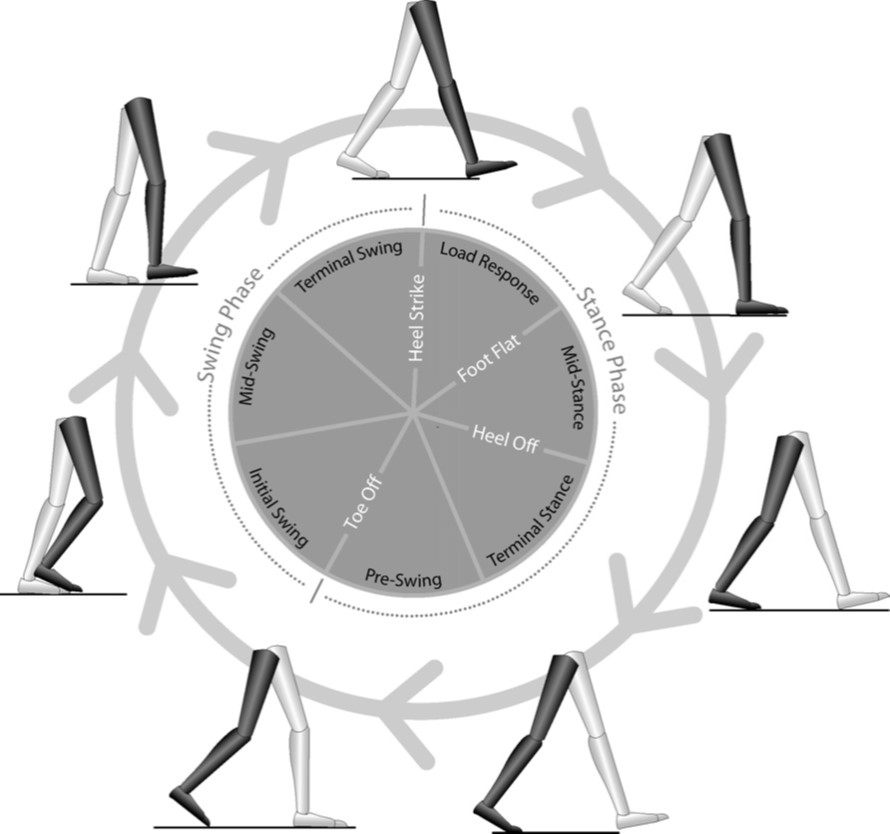
\includegraphics[width=\textwidth,height=\textheight,keepaspectratio]{Figures/gait_event_whittle.jpg}
\decoRule
\caption[Gait event definition]{Gait events as defined in \cite{Whi06}}
\label{fig:gait_event_whittle}
\end{figure}
\noindent
There are various gait event detection methods with different types of sensors and sensor configurations. This is well-documented in a meta-analysis by \cite{Rue10}. In most cases, recent research on gait analysis utilize either force-based sensor, IMU sensor, magnetometer or some combination of aforementioned devices to detect gait events. While it is also possible to obtain gait events from motion capture systems such as the VICON or from depth cameras, these devices are overly sophisticated for the sole purpose of gait event detection.
\\\\
Force-based sensors which measure ground reaction force, range from simple on-off switches to pressure sensitive sensors either in a standalone mat form factor or embedded within the shoe. MEMS (Micro-Electro-Mechanical Systems) IMU sensors and magnetometers are often packaged onto a single board and measure acceleration, angular velocity and magnetic field. Acceleration data is well suited for detecting shocks resulting from contact such as the heel-strike event. For functional analysis angular velocity data is preffered as angular velocity magnitude is invariant to sensor placement, under the reasonable assumption that the sensor is attached to a rigid body (i.e. shoe). Magnetometers can be prone to local magnetic disturbances, especially so in an indoor settings and must be used with caution. Detailed description of gait event detection using IMU sensors is presented by \cite{Jas06}.
\\\\
Different techniques can be deployed to detect gait events from sensor data.  \cite{Rue10} presents a summary of commonly used gait detection methods. With force-based sensors simple thresholding can get the job done. In many cases, functional analysis of either raw sensor data or derived data coupled with FSM (Finite State Machine) can provide reliable gait event detection. With the recent explosion of various learning techniques, data-driven approach  can outperform traditional techniques in some cases.

%-----------------------------------
%	SUBSECTION 2
%-----------------------------------

\subsection{Gait Feature Extraction}
Gait features can be classified into two categories: spatio-temporal and kinematic. The former is represented by a single parameter and the latter is represented by a time series or a waveform. Spatio-temporal features are parameters pertaining to space (spatial) and time (temporal). Spatial parameters include but not limited to step length, stride length, clearances (e.g. MTC, minimum toe clearance), maximum and minimum heights. Temporal parameters include but not limited to cadence, speed and duration between gait events. Kinematic features can be any time series or waveform related to gait that may or may not be represented by wavelets. Kinematic features include but not limited to time series of joint angles, limb angular velocity and limb acceleration.
\\\\
Focusing on IMU-based gait feature extraction techniques, the traditional approach is to obtain gravity-compensated accelerometer data represented in the ground frame with the knowledge of sensor orientation and perform successive integration with constraints provided by gait events to obtain drift-compensated velocity and position \citep{Ram15, Kit16}. Recently there has been data-driven approach to extract gait features directly from IMU sensor data with deep convolutional neural networks \citep{Han17}. If the successive stride vectors can be reliably measured and the initial position is given, PDR (Pedestrian Dead Reckoning) is possible. A detailed overview on this topic is provided by \cite{Woo10}. State of the art PDR algorithm considers heel-strike and toe-off phase and improves upon conventional INS-EKF-ZUPT (Inertial Navigation System - Extended Kalman Filter - Zero Velocity Update) algorithm \citep{Ju16}.
\\\\
For the purpose of this research, spatio-temporal parameters are needed. \cite{Kit16} presents a reliable method to obtain foot trajectory with IMU sensors only. It relies on double integration of the gravity-compensated and orientaion-corrected acceleration with some strong assumptions on the underlying motion to eliminate drift. For gait feature extraction, this research largely adopts the method described in \cite{Kit16}. 

\newpage
%----------------------------------------------------------------------------------------
%	SECTION 3
%----------------------------------------------------------------------------------------

\section{Locomotion Generation in VR}

There are various locomotion generation schemes depending on the input used and the system setup. Inputs include but not limited to gamepad or joystick inputs, headset positional tracking, gesture inputs such as tapping, gaze inputs in stare-to-move and look-down-to-move techniques, WIP (Walking-In-Place) and RDW (Redirected Walking, \cite{Raz01}). A brief taxonomy of techniques is presented by \cite{Nil16} (Figure \ref{fig:taxonomy}).

\begin{figure}[th]
\captionsetup{justification=raggedright,singlelinecheck=false}
\centering
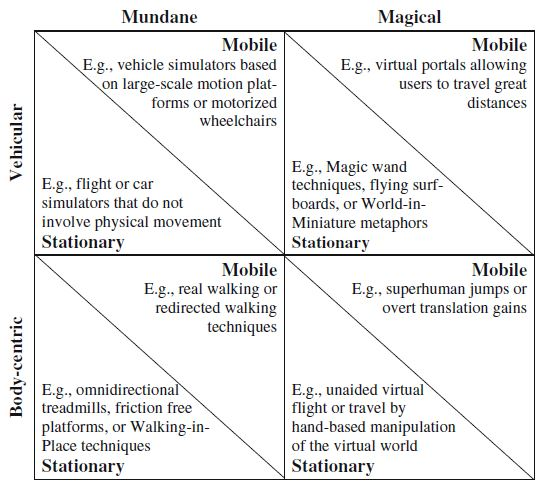
\includegraphics{Figures/taxonomy.jpg}
\decoRule
\caption[Taxonomy of virtual travel techniques]{Taxonomy of virtual travel techniques presented by \cite{Nil16}}
\label{fig:taxonomy}
\end{figure}
\noindent
One of the strong selling points of WIP techniques over headset positional tracking is that the user can navigate infinite virtual space within a limited physical space. Compared with other techniques, WIP techniques provide a interface that is most similar to real walking which is more natural and may alleviate VR sickness. One can argue that RDW which extends the size of the virtual space from a given physical space while retaining the benefits of real walking strikes a nice balance between WIP techniques and headset positional tracking. However, virtual environments have to be designed in such a way that the user following a slightly curved path is convinced to be walking in a straight line without inducing VR sickness. This research seeks to improve upon existing WIP techniques by achieving similar performance with low-cost, inside-out, lightweight IMU-based setup.

\newpage
%-----------------------------------
%	SUBSECTION 1
%-----------------------------------

\subsection{WIP Techniques}
Earlier attempts to synthesize locomotion in VR from WIP motion date back to the 1990s. Surprisingly, earlier attempts include using feed-forward neural networks to determine whether or not the participant is performing WIP motion  \citep{Sla95}. Though the reported accuracy of around 90\% may not be adequate for pratical use. In the last decade there has been resurgence of research on this topic. \cite{Fea08} focused on improving two performance criterion - latency and smoothness (LLCM-WIP, Low-Latency-Continuous-Motion WIP). This was followed by GUD-WIP (Gait-Understanding-Driven WIP) which aimed to generate actual walking-like velocity profile with the knowledge of gait characteristics \citep{Wen10}. \cite{Bru13} improved upon GUD-WIP by using maximum heel height (amplitude) as a metric of locomotion speed and claims less travel time over long distances and improved accuracy in short distances when compared to GUD-WIP (SAS-WIP, Speed-Amplitude-Supported WIP).
\\\\
LLCM-WIP emphasizes low starting/stopping latency and smoothness of the generated locomotion. Heel height signal of left and right foot is conditioned with numerical differentiation, smoothing, DC-bias removal, scaling, etc. which is then summed to be the locomotion speed. Heel height is obtained from magnetic foot trackers. Orientation of the locomotion velocity vector is determined by the chest-orientation tracker. Such implementation, as mentioned by the authors, is prone to magnetic disturbances.
\\\\
Whereas LLCM-WIP relied on signal conditioning of heel height to generate locomotion, GUD-WIP analyzes gait event sequences of walking motion and WIP motion and comes up with a rather sophisticated FSM-based locomotion scheme. The authors claim a smoother, more natural locomotion over LLCM-WIP. However, due to the inherent limitation of state machines, stopping latency is worse than that of LLCM-WIP. GUD-WIP was implemented with optical trackers.
\\\\
SAS-WIP attempts to improve the user experience of the WIP technique by proving the user with more control over locomotion speed which results in reduced user fatigue and better accuracy. Performance is improved (faster long distance travel and more precise short distance travel) over GUD-WIP. SAS-WIP was also implemented with optical trackers.
\\\\
Recently smartphone-based mobile solutions have emerged. Such solutions require minimal hardware and while they may not be as sophisticated as solutions with dedicated hardware, they are more than capable of performing simple functions. \cite{Tre16} synthesizes gaze-directed locomotion when resulting head bobbing motion from WIP triggers an event. Numerous related software packages exist such as the assets found on the Unity Asset Store with varying degrees of success.

\newpage
%----------------------------------------------------------------------------------------
%	SECTION 4
%----------------------------------------------------------------------------------------

\section{Sensor Fusion Orientation Filter}

Orientation can be obtained from multiple sensor data. Accelerometer data provide pitch and roll angles by measuring the direction of gravitational acceleration. Gyroscope data provide orientation relative to initial configuration by integrating angular velocity. Magnetometer data provide a reference direction for yaw angle. Due to sensor characteristics, each has its own strengths and weaknesses. Orientation obtained from accelerometer data is fast and responsive but cannot provide yaw angle and also prone to disturbances such as linear acceleration. Gyroscope data can provide rotations in all directions but is prone to drifting from the integration process. Magnetometer data provide reference heading but more often than not magnetic disturbances, especially in indoor settings, require special consideration.
\\\\
It is common to combine the data from various sensors with sensor fusion algorithms to obtain responsive and robust orientation. IMU-based sensor fusion algorithms require accelerometer and gyroscope data and is used when absolute heading is not required and slight yaw drift is allowed. MARG (Magnetic Angular Rate Gravity) filters incorporate magnetometer data in addition to IMU data to determine the absolute heading but may under-perform compared to IMU filters under high magnetic noise environments. These filters can be implemented with Kalman filters or their variants which is the most widely used approach. Kalman filters require matrix computation which can be computationally expensive. Quaternion-based, gradient descent based orientation filter has been suggested to overcome this computational disadvantage \citep{Mad11}. In this research, Madgwick's algorithm implemented in C was repackaged into C++ class and used to obtain orientation quaternion from IMU sensor data.

% Methods

\chapter{Methods} % Main chapter title

\label{Chapter2} % Change X to a consecutive number; for referencing this chapter elsewhere, use \ref{ChapterX}

%----------------------------------------------------------------------------------------
%	SECTION 1
%----------------------------------------------------------------------------------------

\section{System Setup}

\begin{figure}[th]
\captionsetup{justification=raggedright,singlelinecheck=false}
\centering
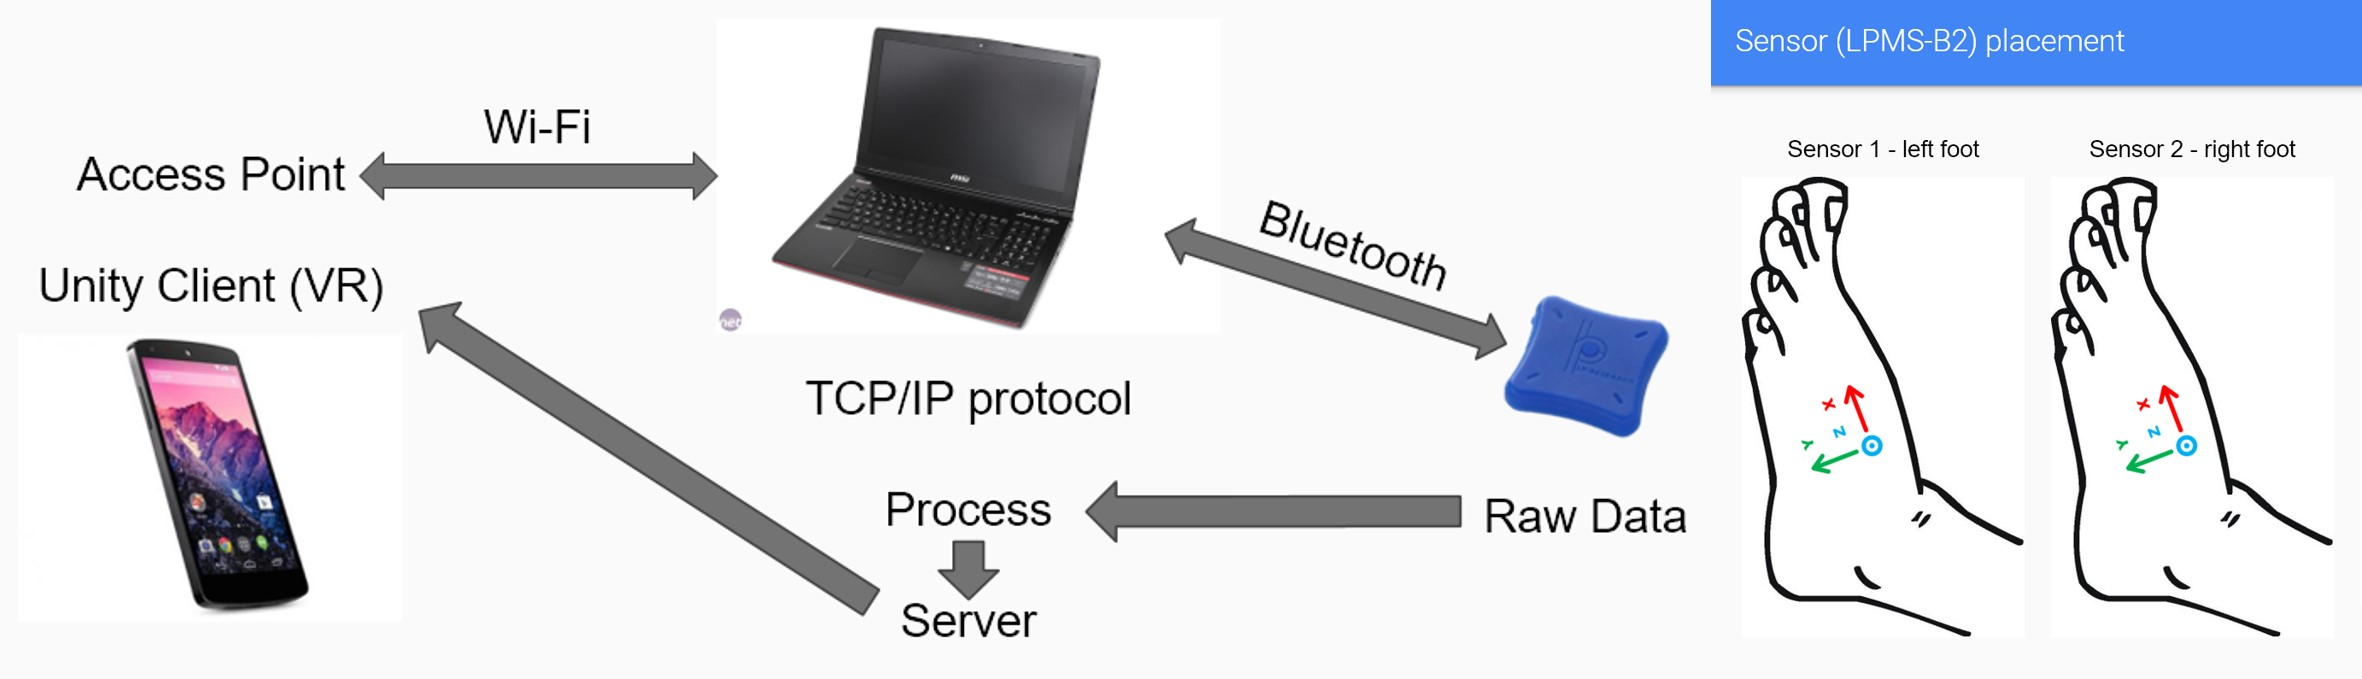
\includegraphics[width=\textwidth,height=\textheight,keepaspectratio]{Figures/system_overview.jpg}
\decoRule
\caption[System overview]{System overview}
\label{fig:system_overview}
\end{figure}
\noindent
System overview is represented in the Figure \ref{fig:system_overview}. System setup consists of a smartphone running Android 6.0 Marshmallow (Nexus 5), a PC running Windows 10 (MSI GE62) and two IMU sensors (LPMS-B2) mounted on each foot as shown in Figure \ref{fig:sensor_module}. For the purpose of this research, IMU sensors are configured to run at 100Hz sampling rate with gyroscope range of 2000$^{\circ}/s$ and accelerometer range of 8G. Though it should be noted that sampling rate of 200Hz is achievable under current configuration. Refer to the datasheet from the manufacturer for detailed specifications. PC acts as a central hub, processing the data received from the IMU sensors and sending the virtual velocity to the smartphone (VR headset). PC and smartphone is connected by Wi-Fi with smartphone providing connection via hotspot and IMU sensors are connected to PC with Bluetooth. Software was developed on Visual Studio 2015 and tested on Unity 5.6.1f1 with sample VR scenes from Udacity. Google Cardboard enables Unity VR projects to run on smartphones running Android 4.4 KitKat or above.  
\\\\
There are three processes - WIP client, Unity client and server. Algorithm presented in this paper is implemented in the WIP client which processes data from IMU sensors and generates virtual velocity. Unity client receives said velocity from the WIP client and displays the virtual environment accordingly. Server maintains a communication session between WIP client and Unity client. WIP client and server runs on the PC and Unity client runs on the smartphone. WIP client is implemented in C++ and the rest is implemented in C\#.

\begin{figure}[th]
\captionsetup{justification=raggedright,singlelinecheck=false}
\centering
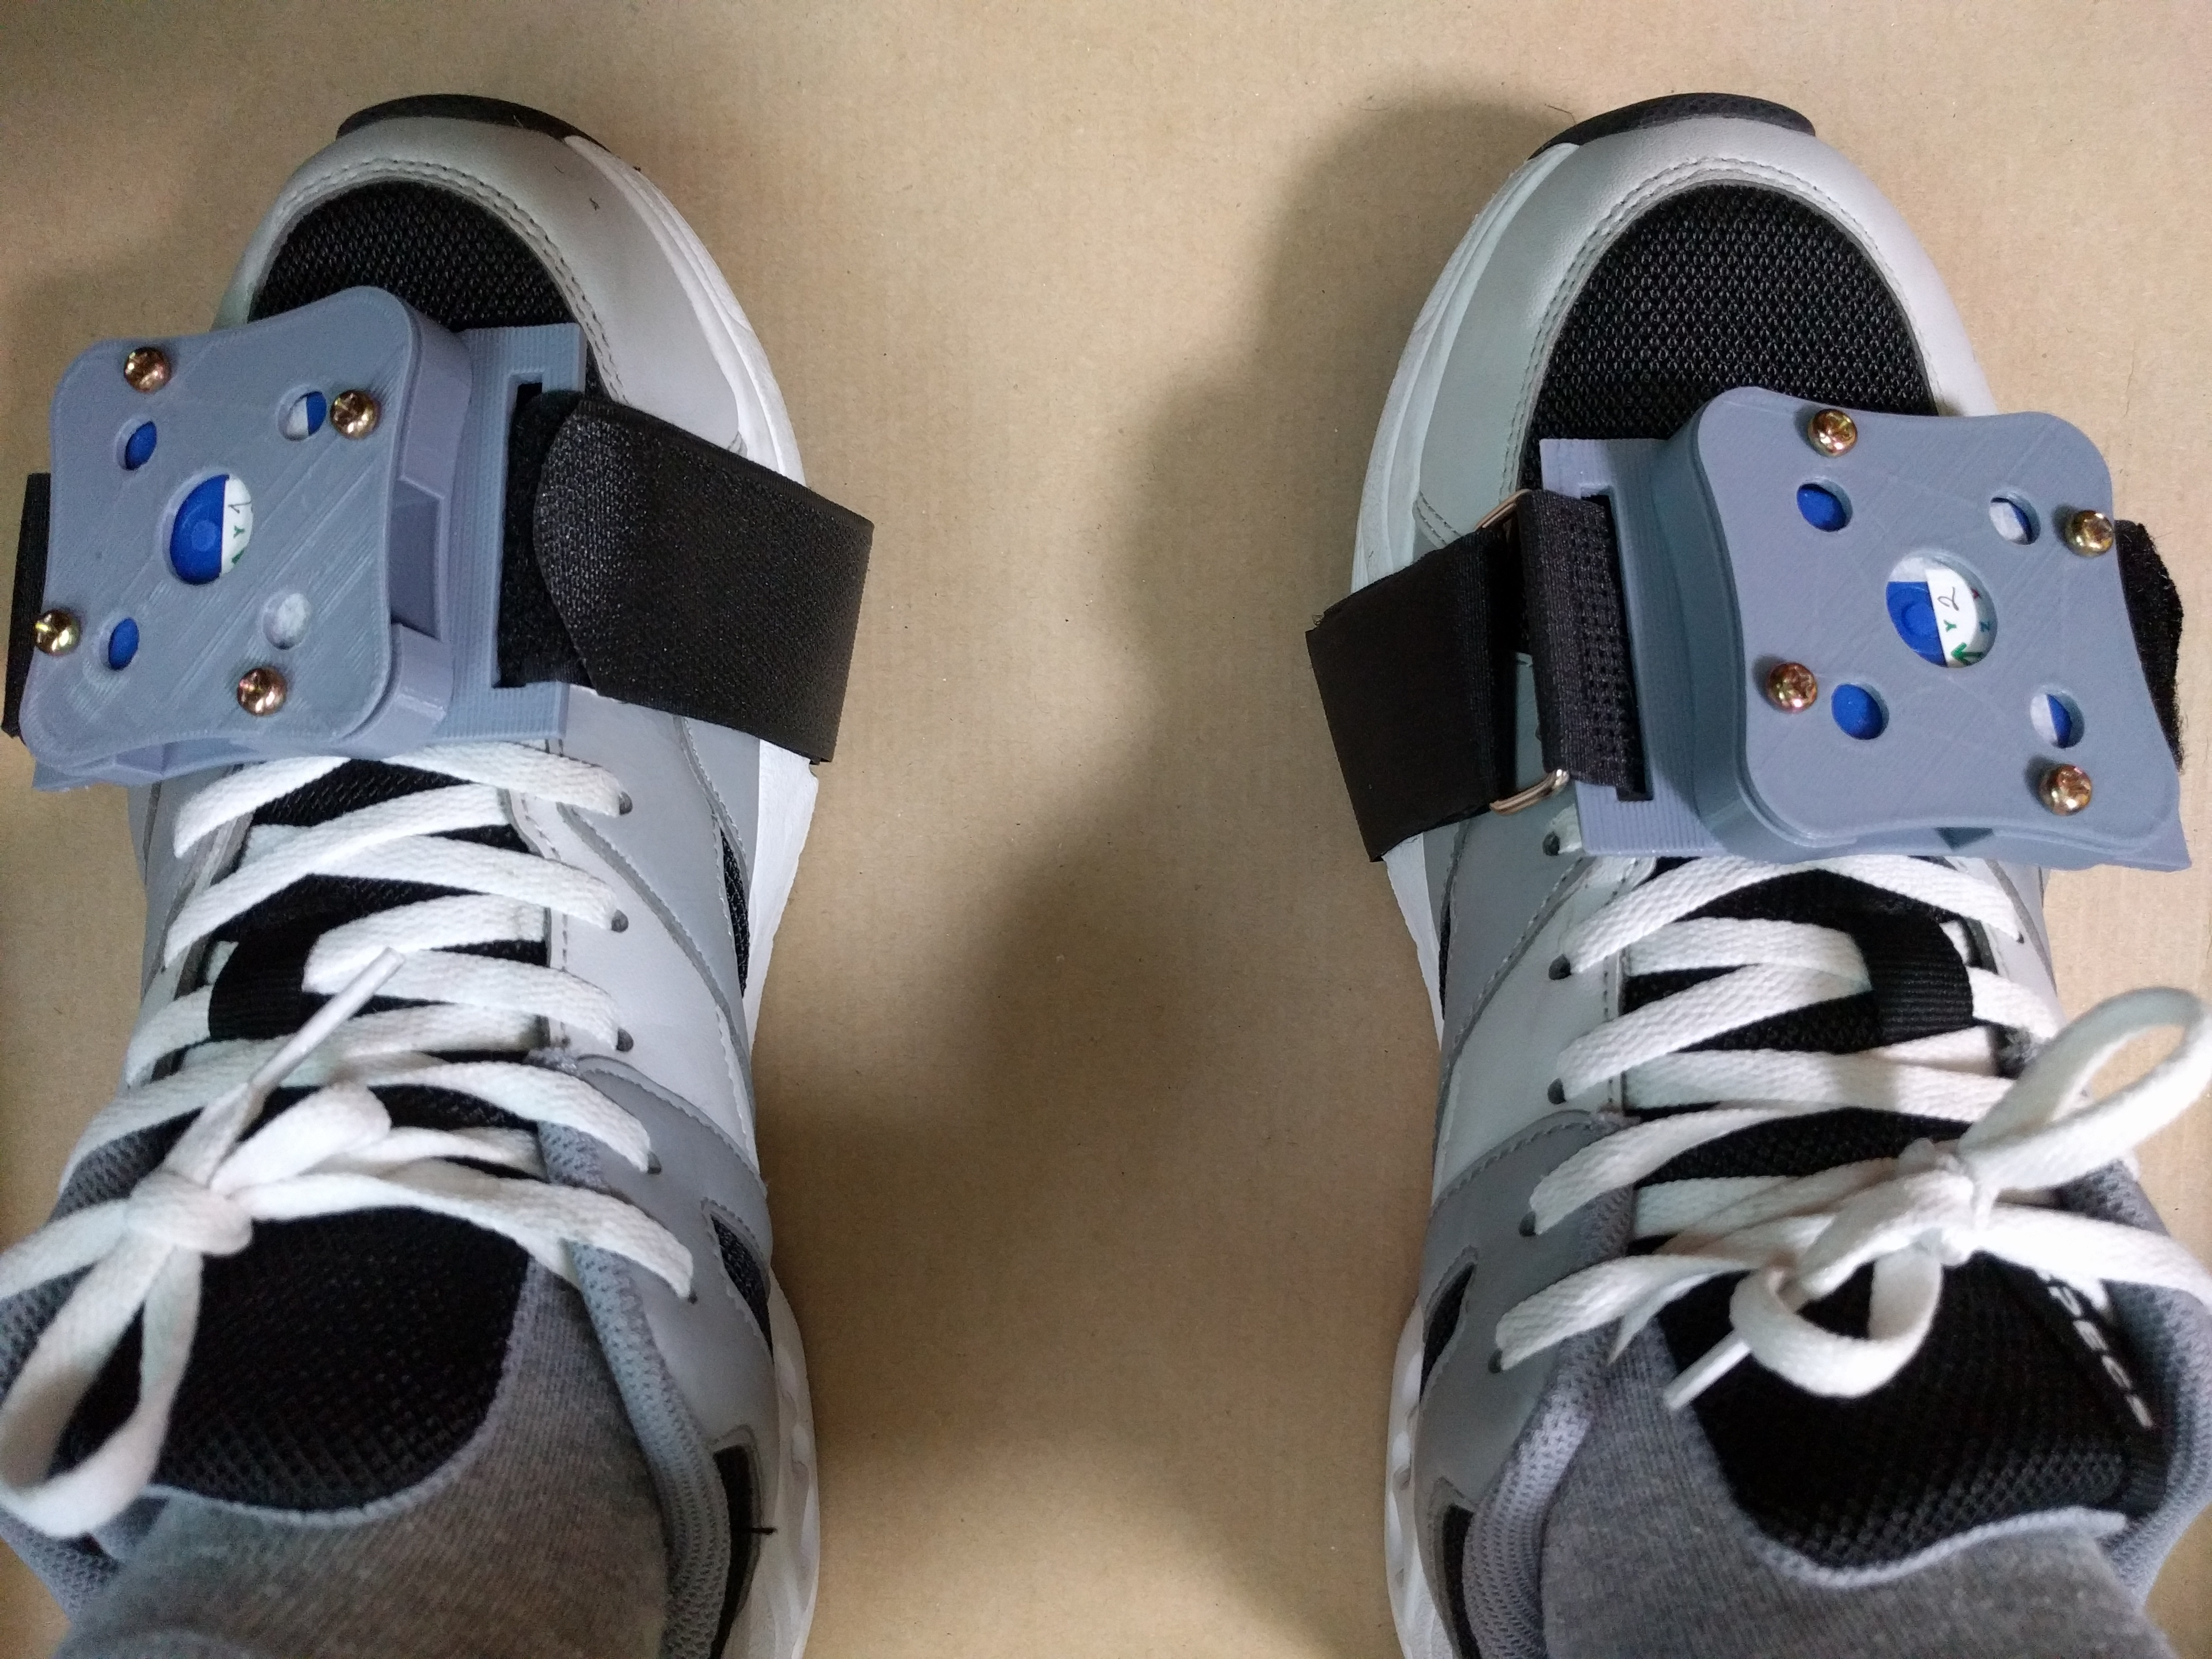
\includegraphics[width=150pt,height=\textheight,keepaspectratio]{Figures/sensor_module.jpg}
\decoRule
\caption[Sensor module with custom brackets]{Sensor module with custom brackets}
\label{fig:sensor_module}
\end{figure}

%----------------------------------------------------------------------------------------
%	SECTION 2
%----------------------------------------------------------------------------------------

\section{Offline Gait Analysis}

Offline gait analysis consist of two parts - event detection and tracking. Gait event detection is implemented with custom FSM (Finite State Machine) with four states and five transitions. Gait tracking borrows from \cite{Kit16} with minor modifications. Gait event detection was not necessary in implementing WIP technique and has been used as a reference only. Kitagawa's algorithm is implemented in the WIP client and executed with 'kita' command (on pre-recorded dataset) or 'calibrate' command (on current recording session).

%-----------------------------------
%	SUBSECTION 1
%-----------------------------------
\subsection{Event Detection}

\begin{figure}[th]
\captionsetup{justification=raggedright,singlelinecheck=false}
\centering
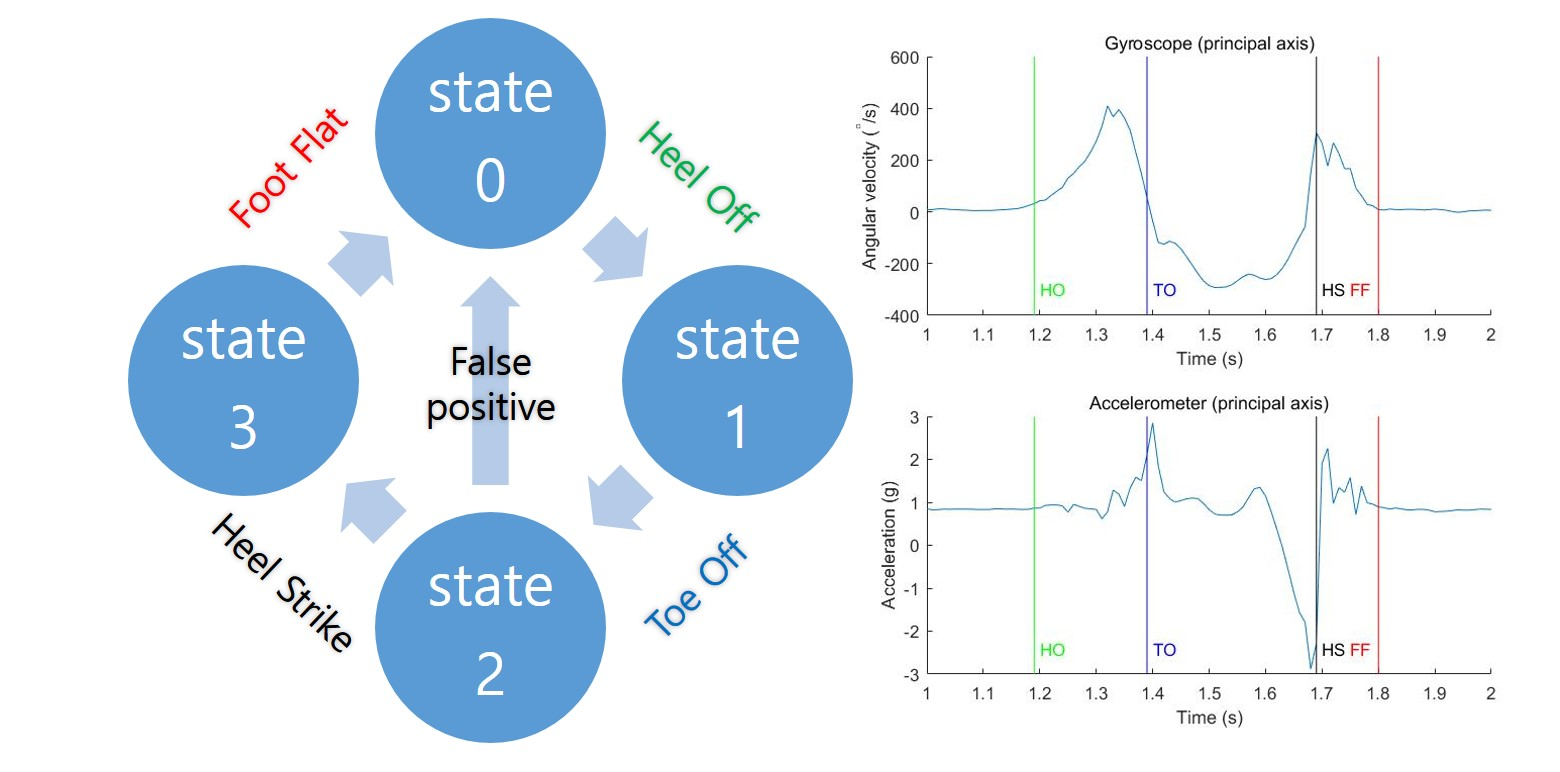
\includegraphics[width=\textwidth,height=\textheight,keepaspectratio]{Figures/gait_event_detection.jpg}
\decoRule
\caption[Gait event detection]{Gait event detection (Right: FSM diagram, Left: gait events superimposed on acceleration and angular velocity along the principal axis)}
\label{fig:gait_event_detection}
\end{figure}
\noindent
Gait event detection relies on gyroscope data only. This is because acceleration can vary depending on sensor placement but angular velocity is independent of sensor placement under the rigid body assumption. Angular velocity along the principal axis, which is defined as the one of the three sensor axes with the largest range of angular velocity, was used to determine the states. This provides better results when compared with using the magnitude of angular velocity - which ensures coordinate invariance - without adding too much complexity. For optimal results it is recommended to roughly align one of the sensor axes to the ankle joint axis. 
\\\\
FSM was devised with functional analysis of the principal axis angular velocity time series (Figure \ref{fig:gait_event_detection}). Initial state (i.e. foot is stationary) is state 0. Transition from state 0 to state 1 occurs when heel-off event is detected. Heel-off event is defined as when the angular velocity exceeds 30$^{\circ}/s$ and is increasing with time. Toe-off event, which is defined as when zero crossing has occurred and the time derivative is less than -2000$^{\circ}/s^{2}$, triggers the transition from state 1 to state 2. Two transitions are defined for state 2. Transition to state 3 occurs when heel-strike is detected. Heel-strike is defined as when zero crossing in the other direction has occurred and the time derivative is greater than 2000$^{\circ}/s^{2}$. Transition to state 0 occurs when there is a false positive and gait is not recognized. This condition is satisfied to be when the angular velocity is greater than zero for certain time steps prior to heel-strike. Foot-flat event, which is defined as when angular velocity is below 10$^{\circ}/s$, triggers the transition from state 3 to state 0. The sign of the principal angular velocity might have to be flipped to match the graph in Figure \ref{fig:gait_event_detection} if the sensor placement does not follow the one shown in Figure \ref{fig:system_overview}.

%-----------------------------------
%	SUBSECTION 2
%-----------------------------------
\subsection{Tracking}

\begin{figure}[th]
\captionsetup{justification=raggedright,singlelinecheck=false}
\centering
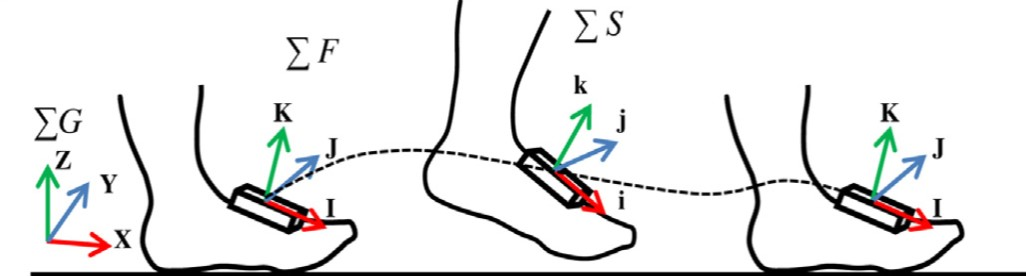
\includegraphics[width=\textwidth,height=\textheight,keepaspectratio]{Figures/kitagawa.jpg}
\decoRule
\caption[Kitagawa's method]{Figure from \cite{Kit16}. Ground frame G is fixed to the ground. Sensor frame S is fixed to the sensor and F is the sensor frame at foot-flat.}
\label{fig:kitagawa}
\end{figure}
\noindent
Gait tracking algorithm follows the method described in \cite{Kit16} but implemented with quaternions instead of rotation matrices for coordinate transformations. Kitagawa's method performs double integration with velocity and position drift correction for accurate gait trajectory tracking. From the gait trajectory, spatio-temporal gait features can be extracted. For detailed description of the algorithm, refer to Kitagawa's paper. A summary is provided below. 
\\\\
1. Find foot-flat and foot-off time with simple thresholding of angular velocity to obtain $T_{0}$ and $T_{f}$.\\
2. Save acceleration $a_{F0}$ (gravity) and orientation quaternion $q^{F}_{G}$ at $T_{0}$ .\\
3. Find linear acceleration in G coordinates between $T_{0}$ and $T_{f}$.\\
\indent
a. Represent raw sensor acceleration in F coordinates ($a_{Ft}$).\\
\indent
b. Subtract $a_{F0}$ to obtain gravity compensated linear acceleration.\\
\indent
c. Represent said value in G coordinates.\\
4. Integrate linear acceleration by time and apply velocity drift correction such that the velocity is zero at $T_{f}$.\\
5. Integrate once more and apply positional drift correction such that the vertical component of position is zero at $T_{f}$.

%----------------------------------------------------------------------------------------
%	SECTION 3
%----------------------------------------------------------------------------------------

\section{Real-time WIP Tracking}

Real-time WIP tracking can be difficult due to the real-time aspect. Unlike offline analysis where the entire time series is available, real-time applications have to work with data up to the current time point. Moreover, system lag and overall latency also becomes an issue for real-time applications. Specifically for tracking WIP in real-time, estimating velocity drift rate which affects the tracking accuracy of the consequent step is crucial. This can be done by taking into account the history of past velocity drift rates with a feedback loop. With the feedback loop in place complications such as ensuring the stability of the system arise.

%-----------------------------------
%	SUBSECTION 1
%-----------------------------------
\subsection{FSM}
%WIP event detection is implemented with BSM (Binary State Machine) which relies on IMU data with simple threshold functions. In order to improve system latency, orientation quaternion relative to foot-flat orientation is decomposed into xy rotation and z rotation components which is then converted into axis-angle representation to be processed with threshold function.

\begin{figure}[th]
\captionsetup{justification=raggedright,singlelinecheck=false}
\centering
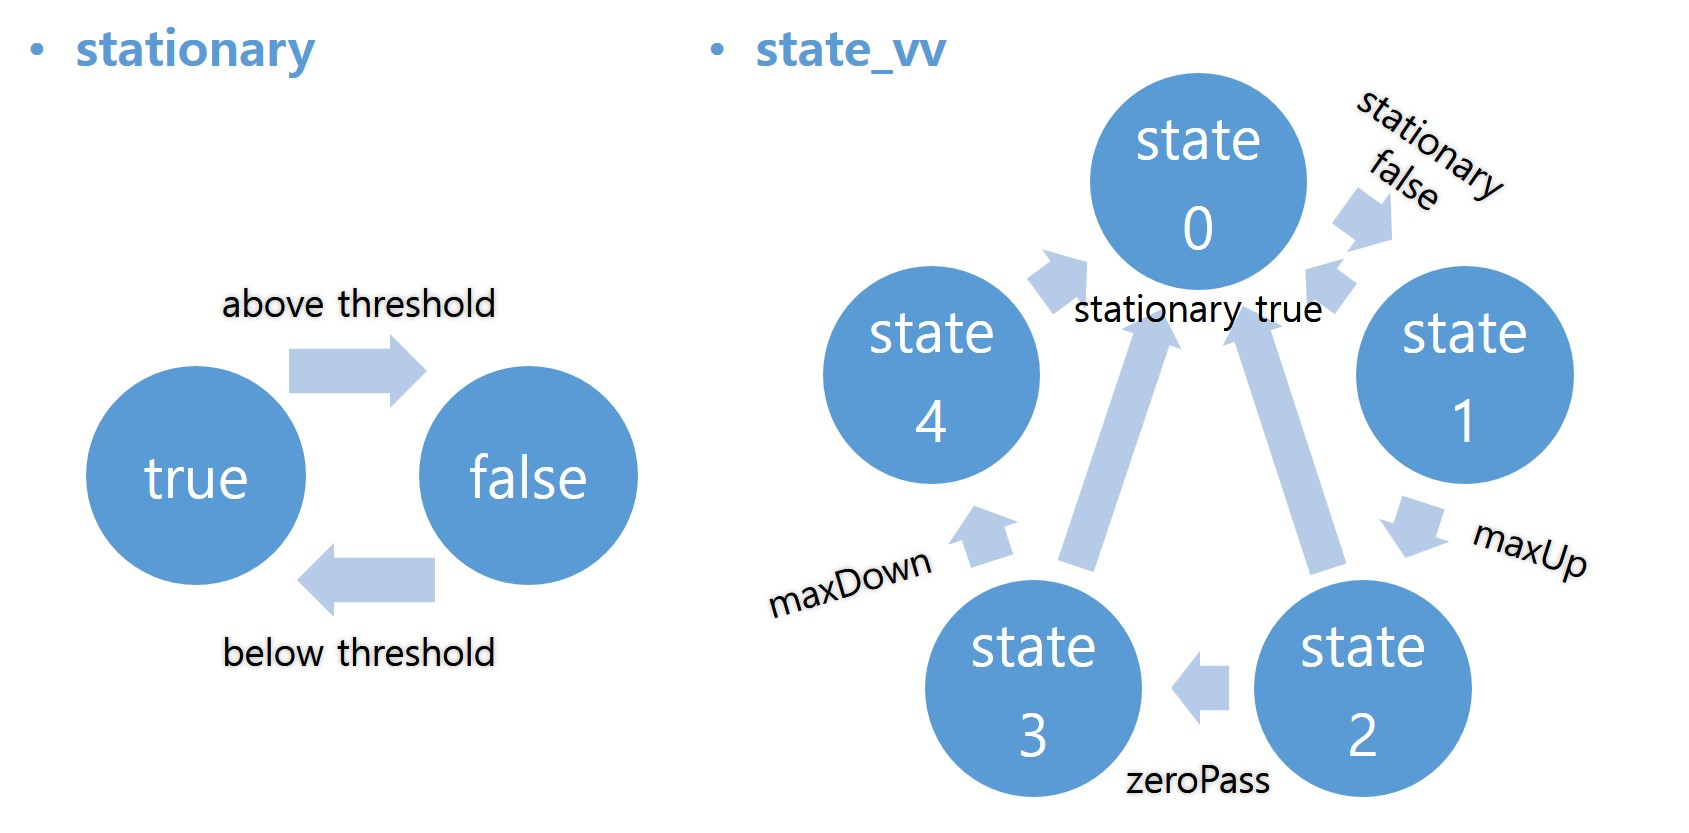
\includegraphics[width=\textwidth,height=\textheight,keepaspectratio]{Figures/WIP_FSM.jpg}
\decoRule
\caption[FSM diagram for WIP motion]{FSM diagram for WIP motion (Left: stationary, Right: state\_vv)}
\label{fig:WIPFSM}
\end{figure}
\noindent
There are two FSMs for real-time WIP motion tracking as shown in Figure \ref{fig:WIPFSM}. FSM for stationary utilizes simple thresholding for state transition. Thresholding is performed on band-pass filtered acceleration and low-pass filtered angular velocity. If the filtered values are under the user configurable thresholds, foot is assumed to be stationary. Through trial and error optimal threshold was set as 0.04G and 30$^{\circ}/s$ for acceleration and angular velocity thresholds, respectively. Band-pass filter for acceleration was implemented as subtracting known offset of 1G (gravity) from raw acceleration magnitude which was then processed with first order digital IIR (Infinite Impulse Response) low-pass filter with a cutoff frequency of 5Hz and a sampling rate of 100Hz.
\\\\
FSM for state\_vv was devised with functional analysis of the vertical component of the foot velocity. Under WIP motion, foot travels up and down resulting in a vertical velocity profile that is sine-like. When foot is stationary, state\_vv is at state 0. Otherwise state\_vv follows a clockwise state transition triggered by events maxUp, zeroPass, maxDown (Figure \ref{fig:WIPFSM}). maxUp event is when foot reaches maximum upwards velocity, followed by zeroPass event when the foot reaches the apex  and heads back down. maxDown event is when foot reaches maximum downwards velocity.

%-----------------------------------
%	SUBSECTION 2
%-----------------------------------
\subsection{Position Tracking}
The basic idea behind real-time WIP position tracking algorithm is similar to Kitagawa's method used for gait tracking. However, the real-time aspect introduces some challenges, particularly with drift correction and lag from application of filters in the FSM. Pseudocode of the algorithm is presented below.
\\\\
1. Represent the raw acceleration measured in sensor frame in ground coordinates and subtract gravity (0, 0, 1)G to obtain gravity compensated linear acceleration $a_{G}$.\\
2. During non-stationary periods integrate velocity drift rate corrected linear acceleration by time to obtain velocity in ground coordinates $v_{G}$.\\
3. Integrate once more during non-stationary periods to obtain position in ground coordinates $x_{G}$. If the vertical component of position falls below zero said component is set to zero. Also, during stationary periods $x_{G}$ is set to zero.\\
4. Let $v_{G}$ at transition from non-stationary to stationary be drift velocity $v_{drift}$ and the duration of the last non-stationary session be $\Delta t$. Then the velocity drift rate is updated by the following equation in feedback form.\\\\
\centerline{$\dot{v}_{drift} = \dot{v}_{drift} + v_{drift}/\Delta t$}
\\\\
When compared with Kitagawa's method there is a minor difference in deriving gravity compensated linear acceleration. This is because the definition of $T_{0}$ is complicated to implement in a real-time fashion. Major difference is in drift correction. With real-time tracking it is impossible to know the exact the value of the velocity drift rate beforehand, thus velocity drift rate from the previous session is assumed as the velocity drift rate. This results in reduced accuracy when compared with Kitagawa's method and is a trade-off for running in real-time.

%----------------------------------------------------------------------------------------
%	SECTION 4
%----------------------------------------------------------------------------------------

\section{Locomotion Generation}

A direct and an indirect approach for locomotion generation scheme has been devised. Direct approach reconstructs horizontal velocity of the foot under normal gait from the vertical position of the foot in WIP motion. Simulated horizontal velocity of each foot is then manipulated to generate locomotion in the virtual environment. This approach is largely inspired by the method described in \cite{Fea08} which derives locomotion from signal processing of heel height. Indirect approach generates locomotion from spatio-temporal parameters extracted from WIP motion such as maximum foot height and non-stationary duration. This approach is more in line with recent research such as \cite{Bru13} and \cite{Tre16}.

\newpage
\subsection{Direct Approach}
Direct approach is based on the simple assumption of the WIP motion. One of the simple ways of modelling ankle trajectory during gait is assuming a cycloid trajectory ($t - sin(t)$, $1 - cos(t)$). Then the time derivative of horizontal and vertical component of the cycloid follow $1 - cos(t)$ and $sin(t)$, respectively. Note that the vertical component of the cycloid trajectory and the horizontal component of the time derivative follow the same profile $1 - cos(t)$. Thus, the horizontal velocity of the foot can be reconstructed from vertical position of the foot with an appropriate scale factor. This scale factor can be determined from the results of offline gait analysis. Assuming one-to-one correspondence between vertical components of walking and WIP motion, it is possible to reconstruct horizontal motion from WIP motion. Aforementioned assumptions have been backed with actual data as shown in Figure \ref{fig:cycloid}. Note that the vertical component of walking is not entirely sine-like which is due to the fact that the sensor was mounted at the dorsum of the foot. With reconstructed horizontal motion for both feet, torso velocity is determined by the average of reconstructed feet speeds.
\\\\
\centerline{$v_{z, walking} = V_{z}sin\Big(\dfrac{2\pi}{T}t\Big)$}
\centerline{$v_{r, walking} = V_{r}\Big[1 - cos\Big(\dfrac{2\pi}{T}t\Big)\Big]$}
\centerline{$p_{z, walking} = \int v_{z, walking}dt = \dfrac{TV_{z}}{2\pi}\Big[1 - cos\Big(\dfrac{2\pi}{T}t\Big)\Big]$}\\\\
\centerline{$scale factor = \dfrac{v_{r, walking}}{p_{z, walking}} = \dfrac{2\pi V_{r}}{TV_{z}}$}

\begin{figure}[th]
\captionsetup{justification=raggedright,singlelinecheck=false}
\centering
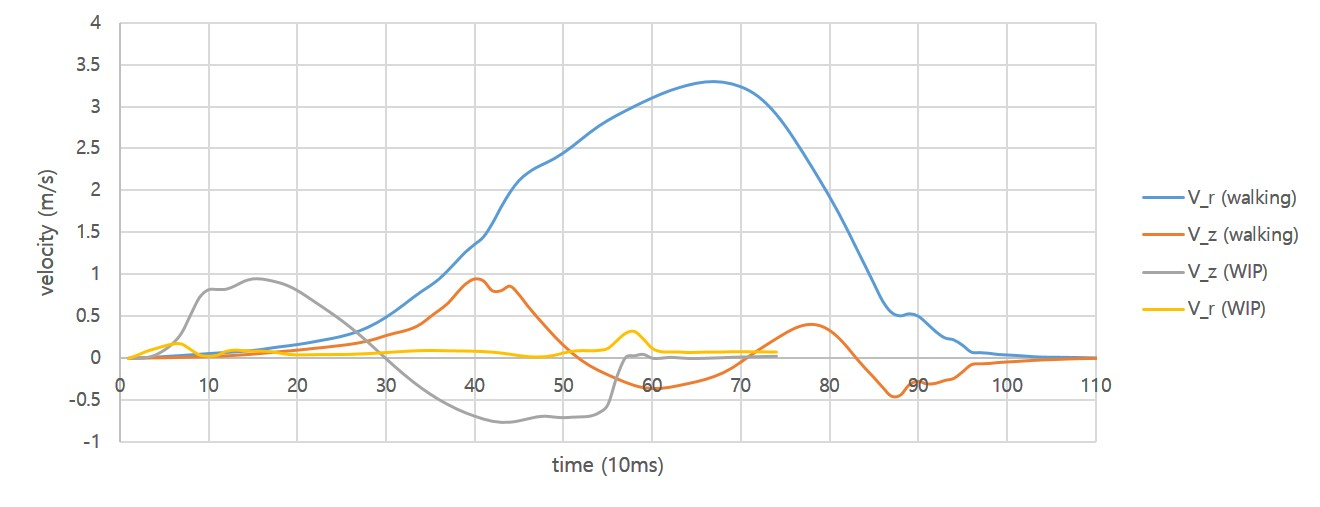
\includegraphics[width=\textwidth,height=\textheight,keepaspectratio]{Figures/cycloid_profile.jpg}
\decoRule
\caption[Sample velocity profile for walking and WIP motion]{Sample velocity profile for walking and WIP motion}
\label{fig:cycloid}
\end{figure}
\noindent
Practical issues arise during implementation. Simple averaging of reconstructed foot motion results in jerkiness. This is due to brief double stance phase causing the motion to abruptly stop midway. Similar issues were discussed by \citep{Fea08} and was mitigated by adopting a low-pass filter to smooth out the locomotion with minor compromise regarding increased stopping latency. In this paper, extra measures were taken to prevent jerkiness and to keep the stopping latency relatively low. When state\_vv is at state 4 ($t_{4}\leq t$), extra padding is applied to prevent speed from falling to zero. The equation is provided below.
\\\\
\indent
$v_{r, reconstructed} = scale factor\times p_{z, WIP}(t)$\indent($t_{1}\leq t\leq t_{4}$)\\
\indent
$v_{r, reconstructed} = 0.5\times scale factor\times (p_{z, WIP}(t) + p_{z, WIP}(t_{4}))$\indent($t_{4}\leq t$)\\
\indent
$v_{locomotion} = 0.5\times(v_{r, reconstructed (left)} + v_{r, reconstructed (right)})$

\subsection{Indirect Approach}
Unlike direct approach, indirect approach does not utilize the entire time series of the foot vertical position. It only requires maximum foot height and non-stationary duration. Higher maximum foot height and shorter non-stationary duration corresponds to faster locomotion. Maximum foot height and non-stationary duration is updated when either one of the foot is at zeroPass (state\_vv transition from state 2 to state 3). The foot is at maximum height at zeroPass and the non-stationary duration is assumed to be double the duration between foot-off and zeroPass. When WIP motion is initiated maximum foot height and non-stationary duration is unknown, thus until one of the feet has reached zeroPass direct approach is used for locomotion. If both feet remains stationary for longer than the user configurable timeout, it is assumed that the user intends to stop. This value will determine the frequency of unintended stops and the stopping latency. In order to distinguish between rotation-in-place and WIP, if maxHeight is under certain threshold (of 0.02-0.03m) speed is set to zero. The equation for indirect approach is presented below.
\\\\
\indent
$v_{locomotion} = scale factor\times maxHeight \times f(WIPPeriod)$,
\\\\
where $f(WIPPeriod)$ is a function that increases as $WIPPeriod$ decreases.

\subsection{Heading}
Locomotion heading can be determined either by user's gaze direction obtained from the headset or by the midway direction of the feet. The latter requires syncing (offset compensation) between the virtual environment frame and the ground frame. Gaze-directed heading is easy to implement as it is provided by the Google Cardboard API. Feet-directed heading needs to be implemented in the WIP client. Pseudocode of said algorithm is provided below.
\\\\
1. Compute relative orientation quaternion to initial orientation quaternion.\\
2. Decompose said quaternion and obtain the two-dimensional direction vector (representing the yaw angle) of both feet.\\
3. Add the direction vector of both feet to obtain midway direction vector.
% Results and Discussion

\chapter{Results and Discussion} % Main chapter title

\label{Chapter3} % Change X to a consecutive number; for referencing this chapter elsewhere, use \ref{ChapterX}

%----------------------------------------------------------------------------------------
%	SECTION 1
%----------------------------------------------------------------------------------------

\section{Offline Gait Analysis}

%-----------------------------------
%	SUBSECTION 1
%-----------------------------------
\subsection{Event Detection}

\begin{figure}[th]
\captionsetup{justification=raggedright,singlelinecheck=false}
\centering
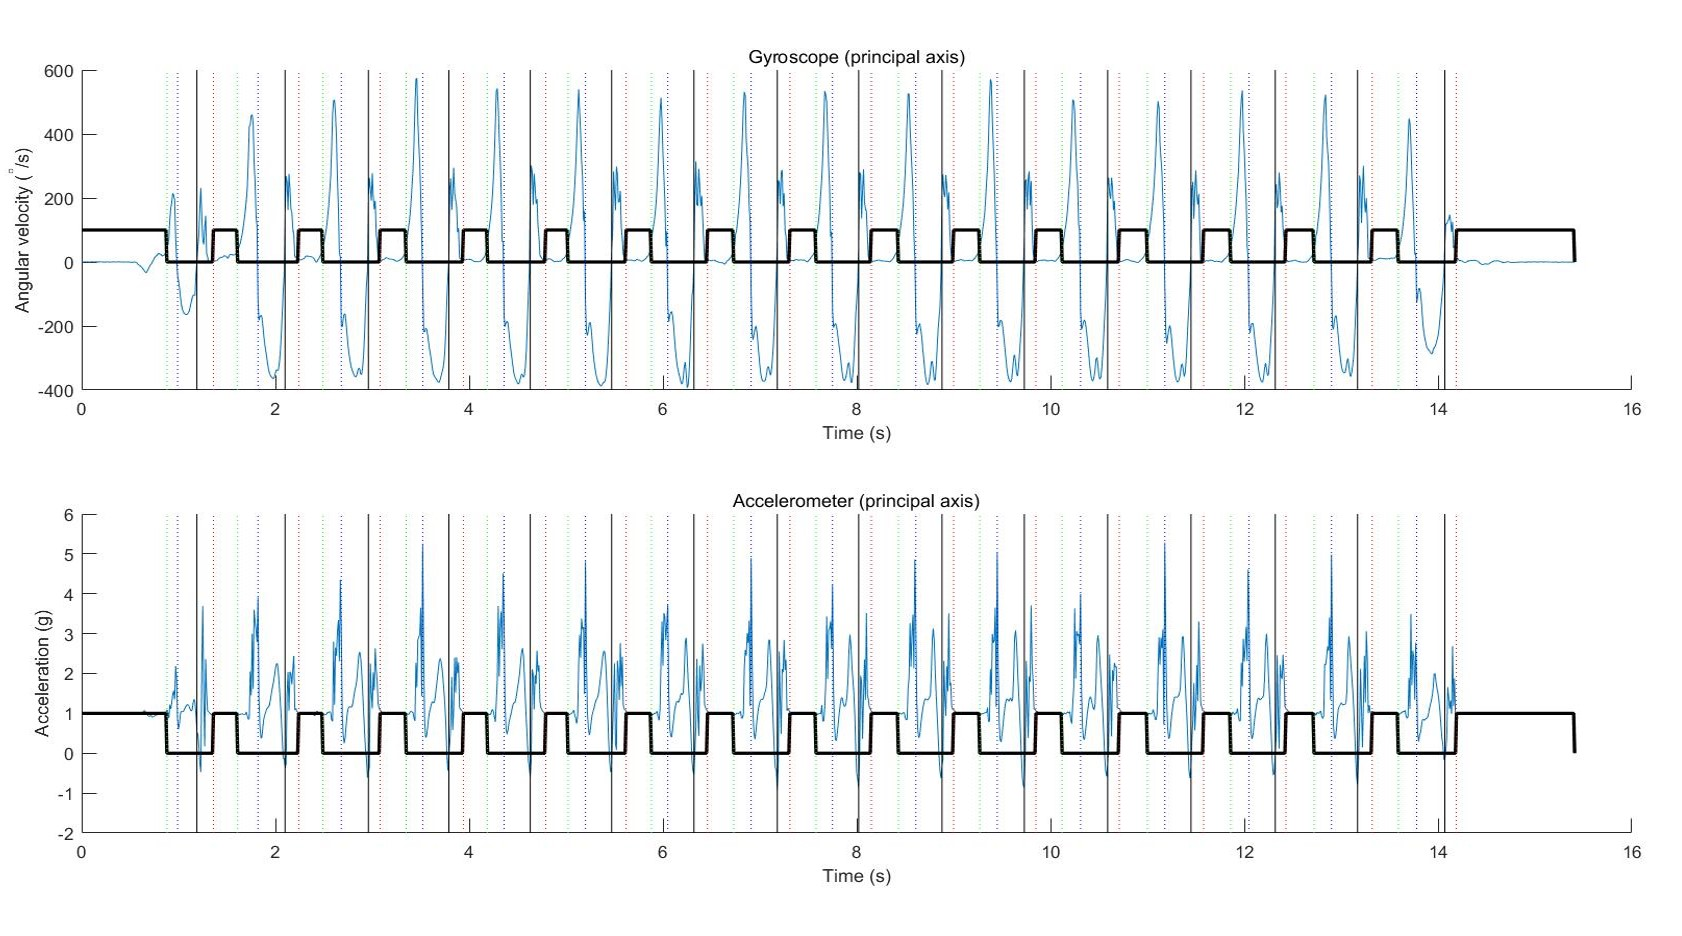
\includegraphics[width=\textwidth,height=\textheight,keepaspectratio]{Figures/gait_event_detection_results.jpg}
\decoRule
\caption[Gait event detection results]{Gait event detection for a sample walking session. Color-coded vertical lines indicate gait events (black: heel-strike, red: foot-flat, green: heel-off, blue: toe-off). Thick black line represents stationary state with zero being stationary.}
\label{fig:gait_event_detection_results}
\end{figure}
\noindent
FSM described in Chapter 2 was used to generate results shown in Figure \ref{fig:gait_event_detection_results}. Gait events were successfully recognized. Gait event detection was only used as a reference and was not required for WIP technique described in this paper.

\newpage
%-----------------------------------
%	SUBSECTION 2
%-----------------------------------
\subsection{Trajectory}

\begin{figure}[th]
%\captionsetup{justification=raggedright,singlelinecheck=false,format=hang}
\captionsetup{justification=raggedright,singlelinecheck=false}
\centering
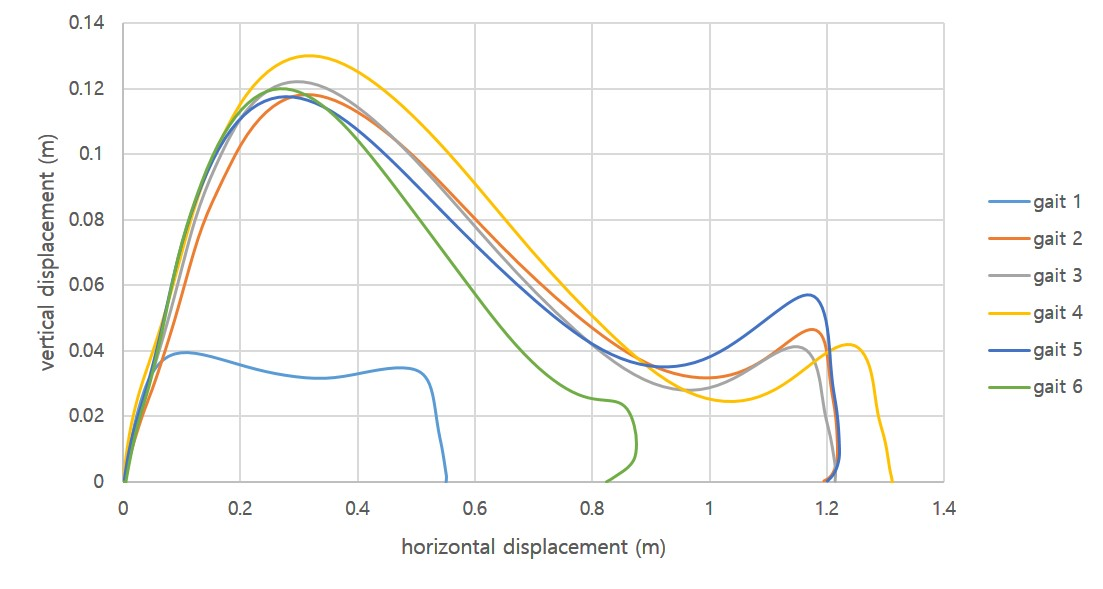
\includegraphics[width=\textwidth,height=\textheight,keepaspectratio]{Figures/gait_feature_extraction_results.jpg}
\decoRule
\caption[Gait feature extraction results]{Gait trajectory for a sample walking session. Gait 1 and 6 are stating and stopping gait sequences, respectively and the rest are steady state gait sequences. Similar results were obtained when compared with \cite{Kit16}.}
\label{fig:gait_feature_extraction_results}
\end{figure}
\noindent
Kitagawa's method summarized in Chapter 2 was used obtain gait trajectory shown in Figure \ref{fig:gait_feature_extraction_results}. Time derivative of the horizontal and vertical component of the trajectory yields $V_{r}$ and $V_{z}$. Period $T$ can also be determined from the results. These parameters provide a baseline for the $scale factor$.

\newpage
%----------------------------------------------------------------------------------------
%	SECTION 2
%----------------------------------------------------------------------------------------

\section{Locomotion Generation}

%-----------------------------------
%	SUBSECTION 1
%-----------------------------------
\subsection{WIP Event Detection}

\begin{figure}[th]
\captionsetup{justification=raggedright,singlelinecheck=false}
\centering
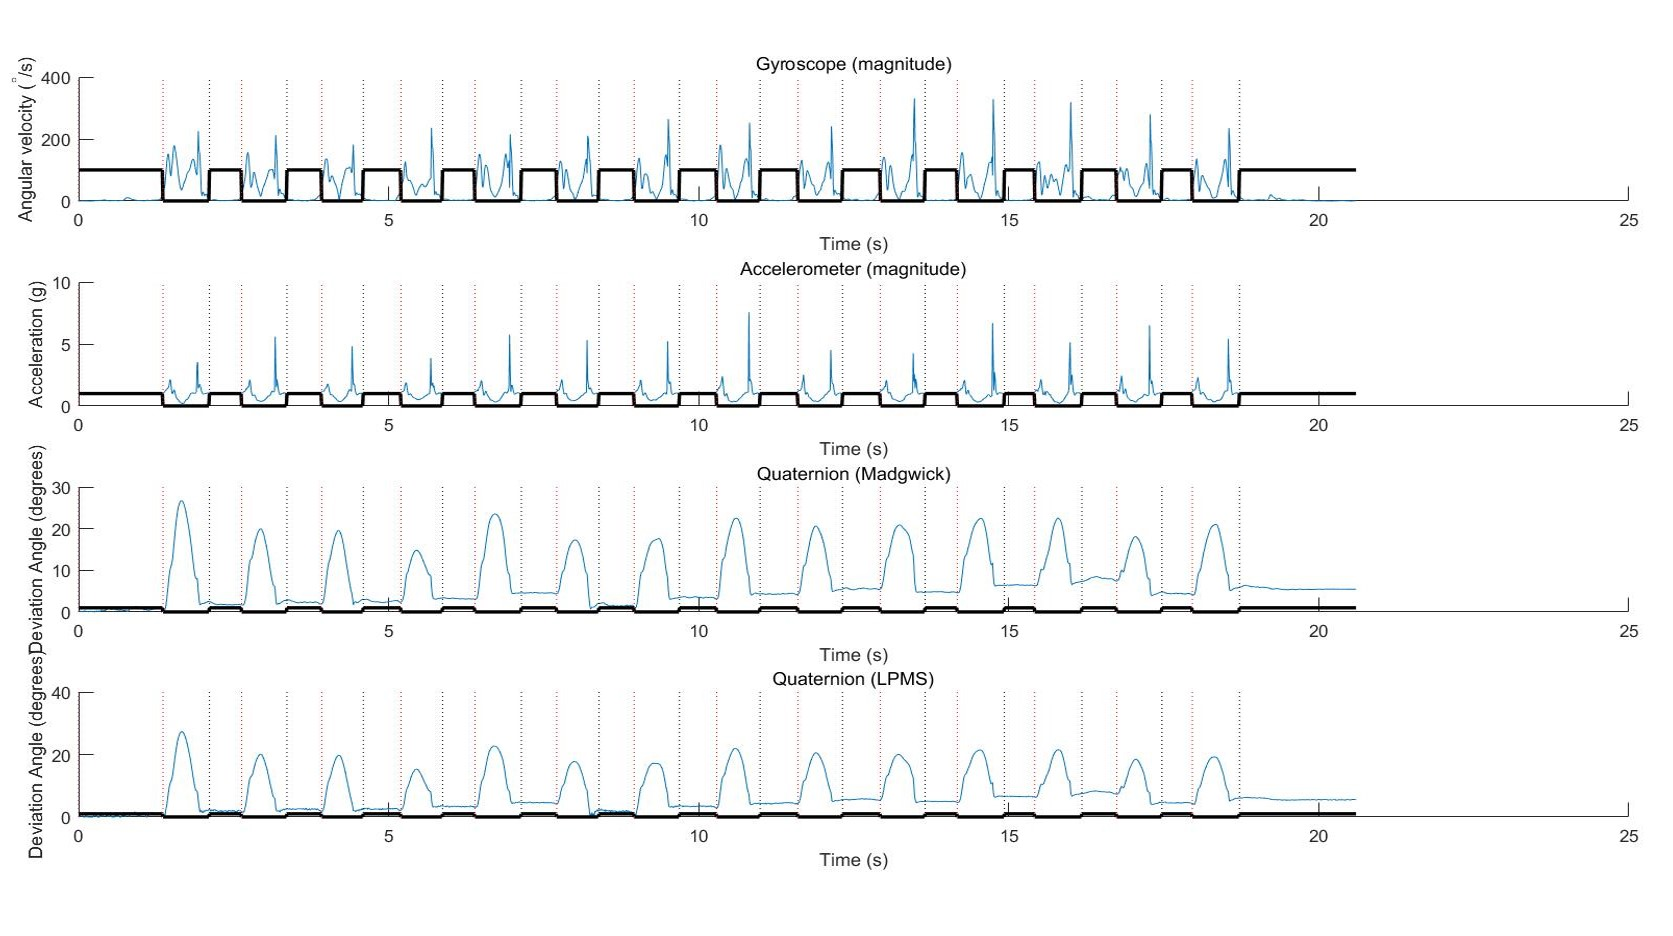
\includegraphics[width=\textwidth,height=\textheight,keepaspectratio]{Figures/wip_event_detection.jpg}
\decoRule
\caption[WIP event detection results]{WIP event detection for a sample WIP session. Color-coded vertical lines indicate state transition (black: foot-strike, red: foot-off). Thick black lines represent stationary state with zero being stationary.}
\label{fig:wip_event_detection}
\end{figure}
\noindent
WIP event detection is shown in Figure \ref{fig:wip_event_detection}. Stationary state is determined by a FSM described in Chapter 2, with simple thresholding for state transition. Deviation angles shown in Figure \ref{fig:wip_event_detection} are derived from axis-angle representation of relative quaternions to initial orientation. In order to verify Madgwick's algorithm, it was compared against quaternion readings from the LPMS-B2 IMU sensor.
\\\\
Figure \ref{fig:wip_quaternion_decomposition} overlays WIP events with xy (pitch and roll) and z (yaw) components of deviation angle. xy component $\phi_{xy}$ and z component $\phi_{z}$ can be obtained from relative quaternion to initial orientation $q = [q_{0},   q_{1},   q_{2},   q_{3}]$ with the following equation.
\\\\
\centerline{$\phi_{z} = 2atan2(q_{3},   q_{0})$ \indent $-\pi\leq \phi_{z}\leq\pi$}
\\\\
\centerline{$\phi_{xy} = 2acos\Big(\dfrac{q_{0}}{cos(\phi_{z}/2)}\Big)$\indent or\indent $2acos\Big(\dfrac{q_{3}}{sin(\phi_{z}/2)}\Big)$ \indent $-\pi\leq \phi_{xy}\leq\pi$}
\\\\
As shown in Figure \ref{fig:wip_quaternion_decomposition}, xy component of deviation angle (in yellow) starts rising right after foot-off event but settles slightly before foot-strike event, suggesting a slight lag in the foot-strike event detection. This is due to use of filtered values for thresholding in the stationary FSM as mentioned in Chapter 2. By adopting xy component of deviation angle as a means of detecting foot-strike event, lag can be reduced at the expense of added complexity of the FSM. However, for the purpose of implementing the WIP technique, slight lag is encouraged to prevent unintended stops in the generated locomotion. Thus, a simple thresholding of filtered acceleration and angular velocity is used for stationary FSM.

\newpage

\begin{figure}[th]
\captionsetup{justification=raggedright,singlelinecheck=false}
\centering
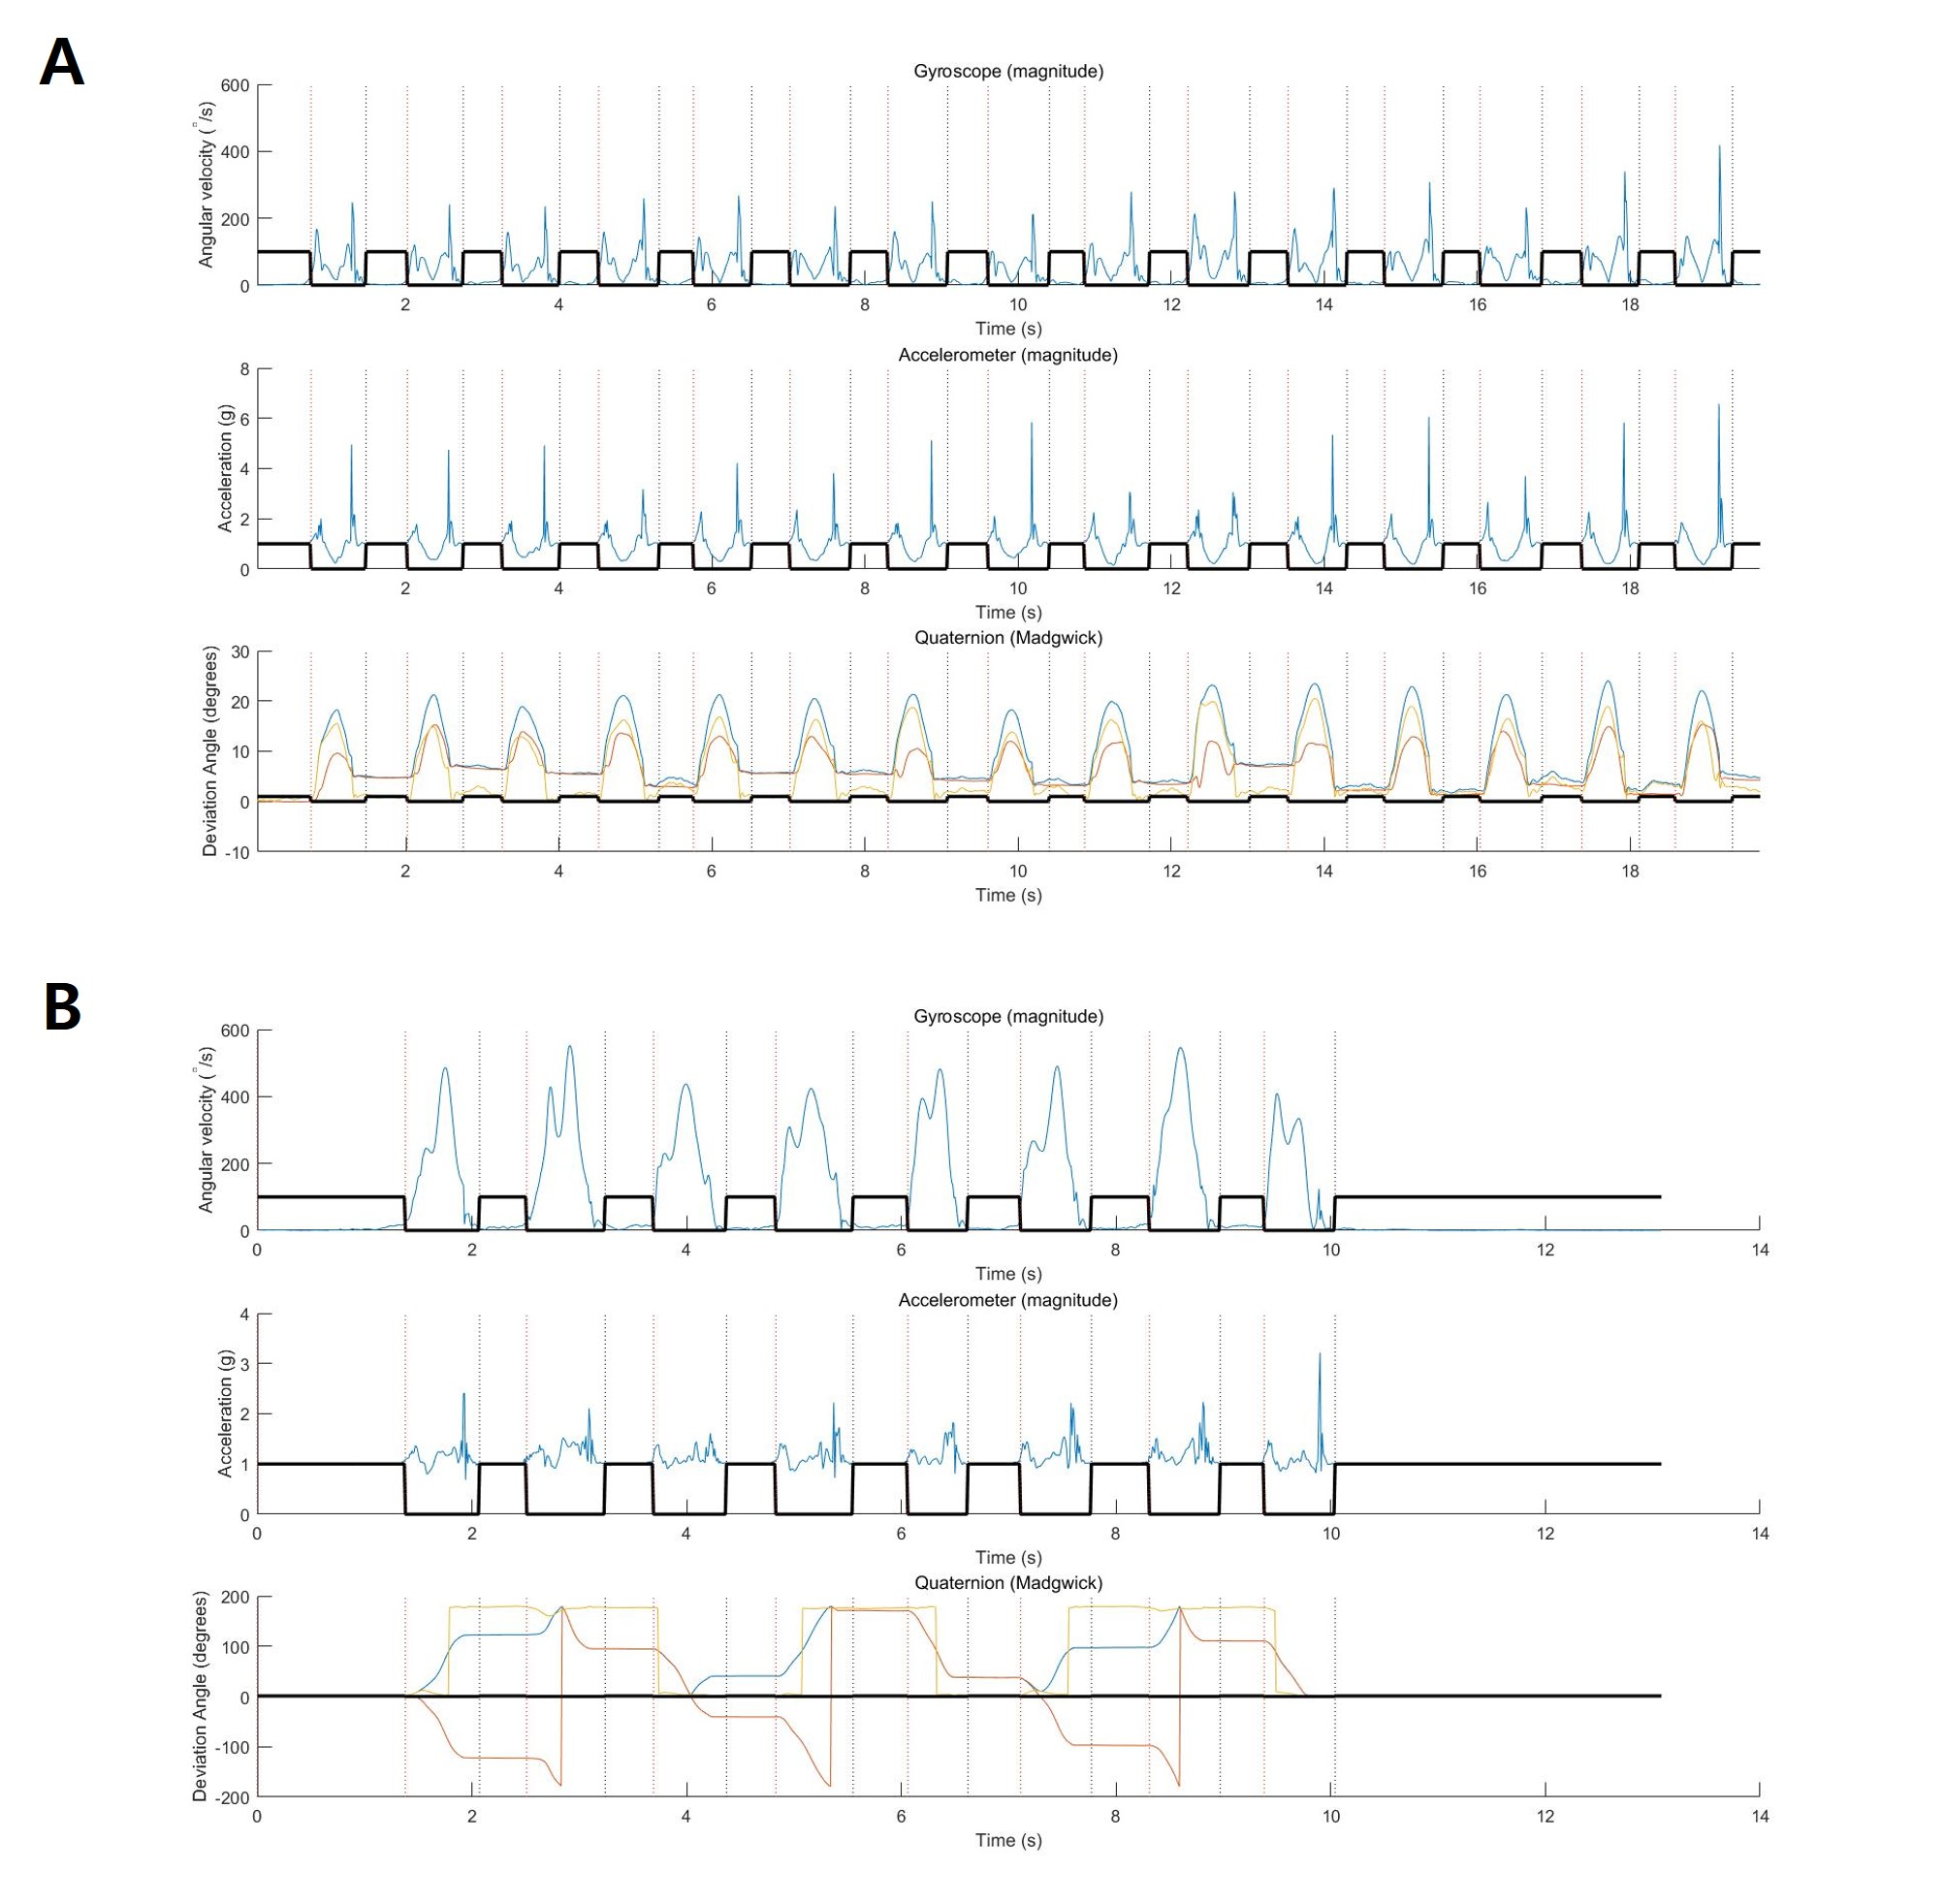
\includegraphics[width=\textwidth,height=\textheight,keepaspectratio]{Figures/wip_quaternion_decomposition.jpg}
\decoRule
\caption[WIP event detection with quaternion decomposition]{WIP event detection for A. simple WIP motion, B. WIP motion with rotation. Color-coded vertical lines indicate state transition (black: foot-strike, red: foot-off). Thick black lines represent stationary state with zero being stationary. Angles obtained from axis-angle representation of the relative quaternions to initial orientation can be decomposed into xy and z component as shown in the third row of A and B (blue: combined, red: z component, yellow: xy component).}
\label{fig:wip_quaternion_decomposition}
\end{figure}
\noindent

%-----------------------------------
%	SUBSECTION 2
%-----------------------------------
\subsection{WIP Sessions}

Direct and indirect approach for locomotion generation was conducted on four different WIP sessions - natural WIP, leisurely WIP, marching WIP and natural WIP with rotation. With offline analysis of gait, the $scale factor$ was appropriately set to generate locomotion that is similar to that of walking. The results are presented in Figure \ref{fig:wip_session1} through \ref{fig:wip_session4}. From the figures it can be seen that the indirect approach maintains identical starting and stopping latencies with the added benefit of reduced jerkiness and the detection of rotation-in-place as seen in Figure \ref{fig:wip_session4}. Demonstration of proposed WIP technique is shown in Figure \ref{fig:demo}.

\begin{figure}[th]
\captionsetup{justification=raggedright,singlelinecheck=false}
\centering
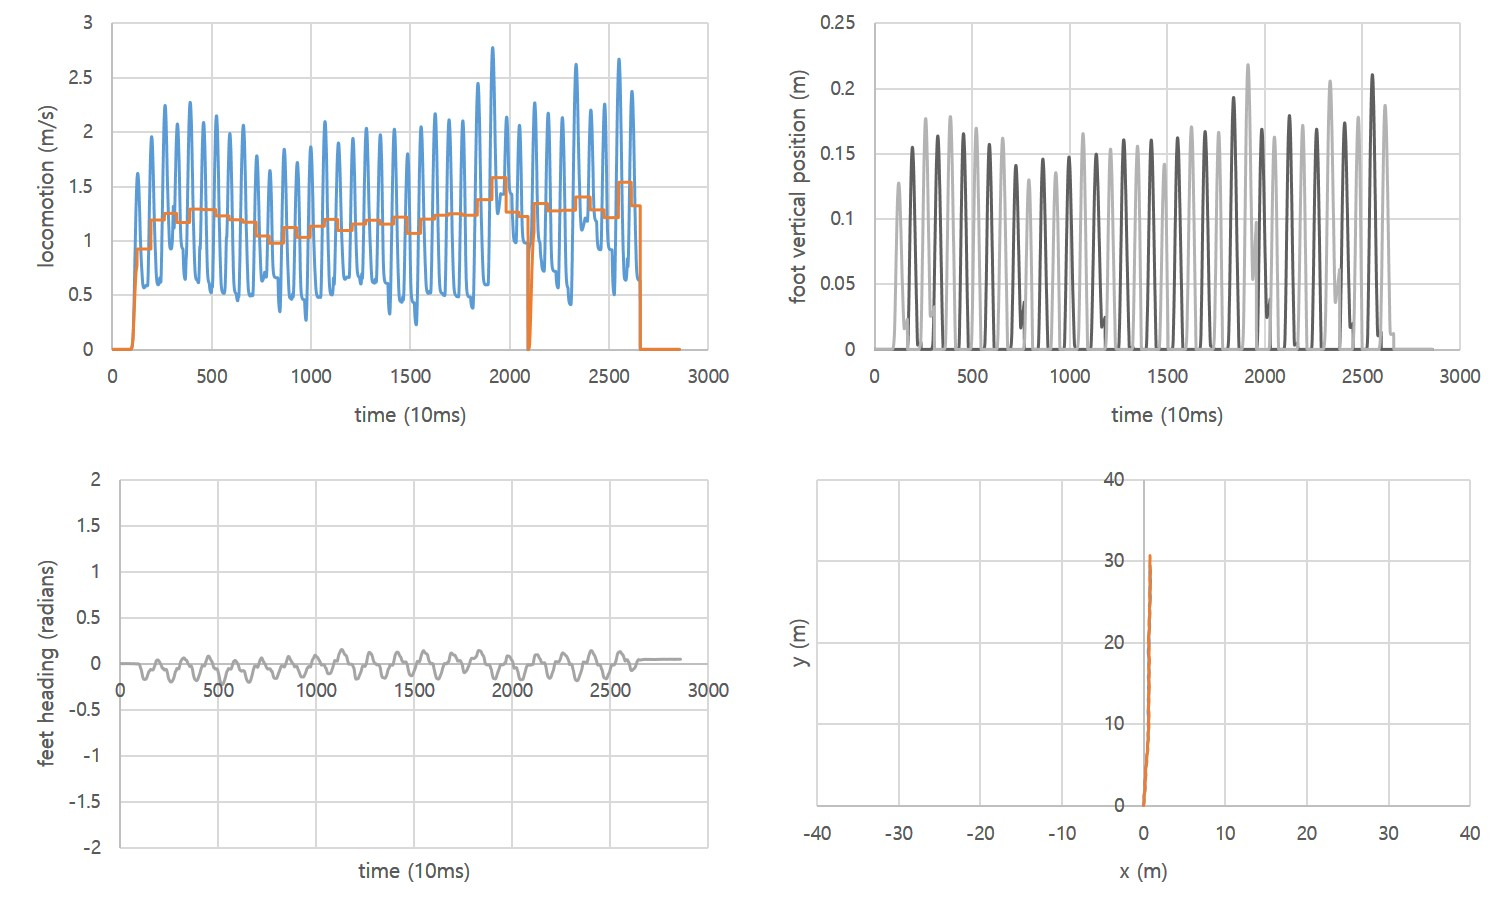
\includegraphics[width=\textwidth,height=\textheight,keepaspectratio]{Figures/session1.jpg}
\decoRule
\caption[WIP session 1]{Locomotion generation for WIP session 1 (natural WIP, medium amplitude). Direct approach is in blue and indirect approach is in orange. Left foot and right foot is in black and grey, respectively.}
\label{fig:wip_session1}
\end{figure}

\begin{figure}[th]
\captionsetup{justification=raggedright,singlelinecheck=false}
\centering
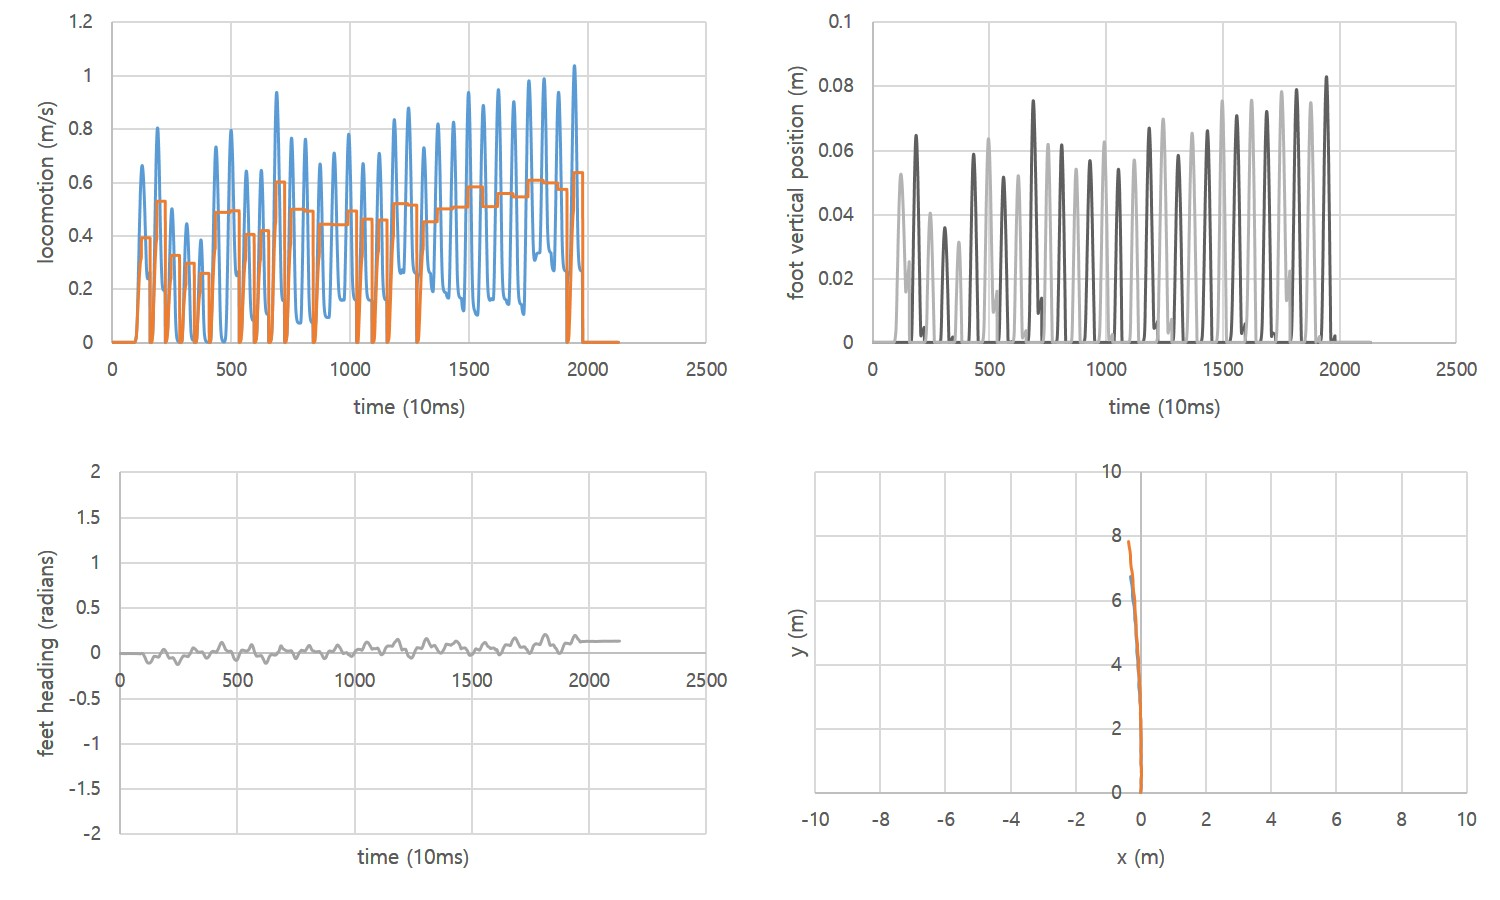
\includegraphics[width=\textwidth,height=\textheight,keepaspectratio]{Figures/session2.jpg}
\decoRule
\caption[WIP session 2]{Locomotion generation for WIP session 2 (leisurely WIP, small amplitude). Direct approach is in blue and indirect approach is in orange. Left foot and right foot is in black and grey, respectively.}
\label{fig:wip_session2}
\end{figure}

\begin{figure}[th]
\captionsetup{justification=raggedright,singlelinecheck=false}
\centering
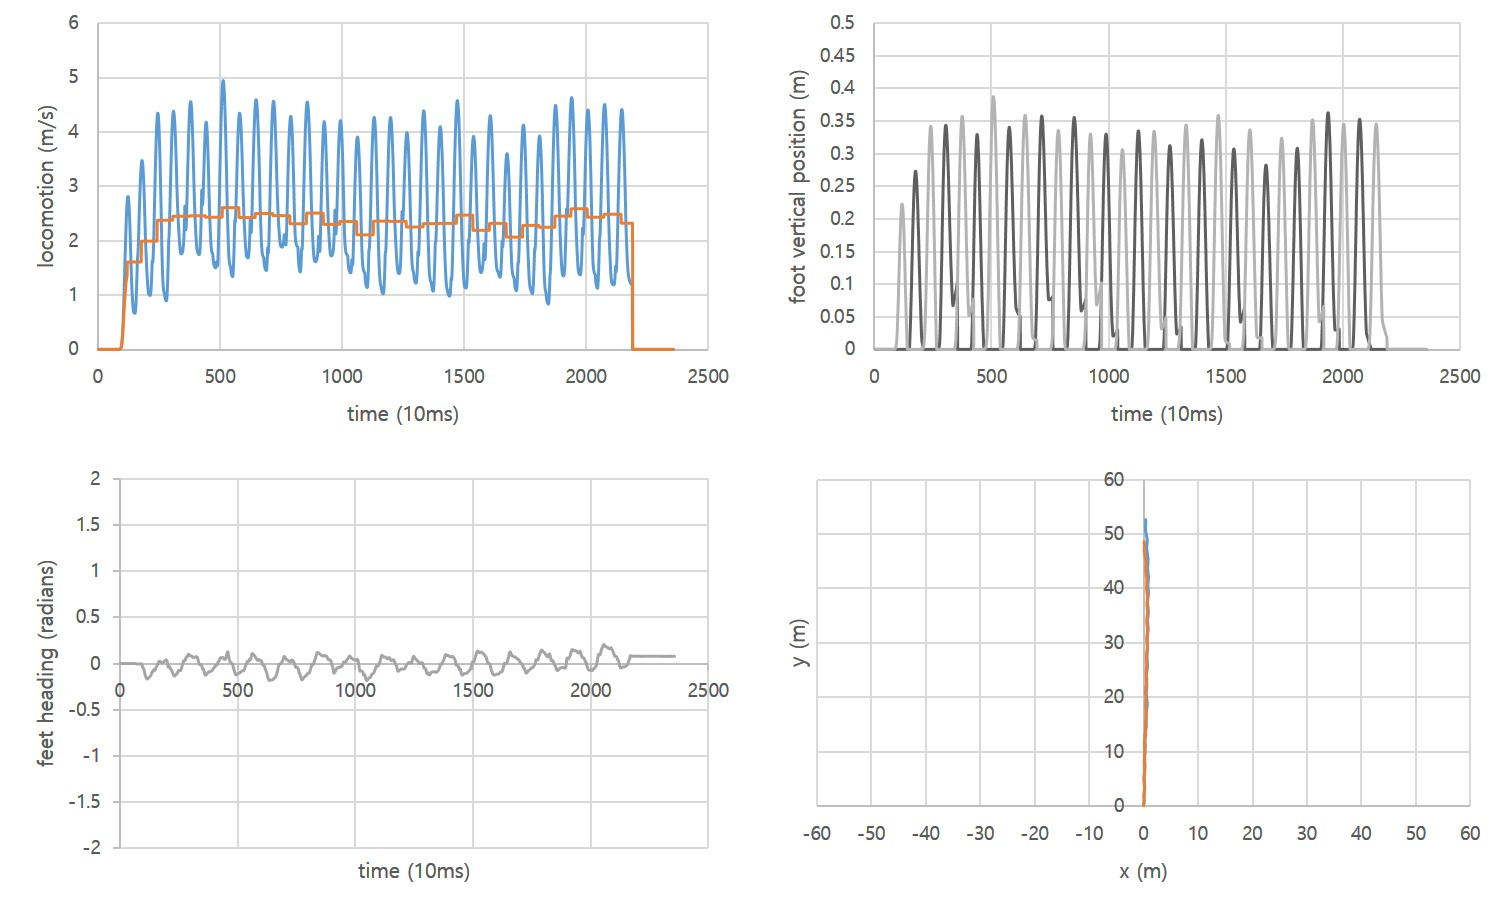
\includegraphics[width=\textwidth,height=\textheight,keepaspectratio]{Figures/session3.jpg}
\decoRule
\caption[WIP session 3]{Locomotion generation for WIP session 3 (marching WIP, large amplitude). Direct approach is in blue and indirect approach is in orange. Left foot and right foot is in black and grey, respectively.}
\label{fig:wip_session3}
\end{figure}

\begin{figure}[th]
\captionsetup{justification=raggedright,singlelinecheck=false}
\centering
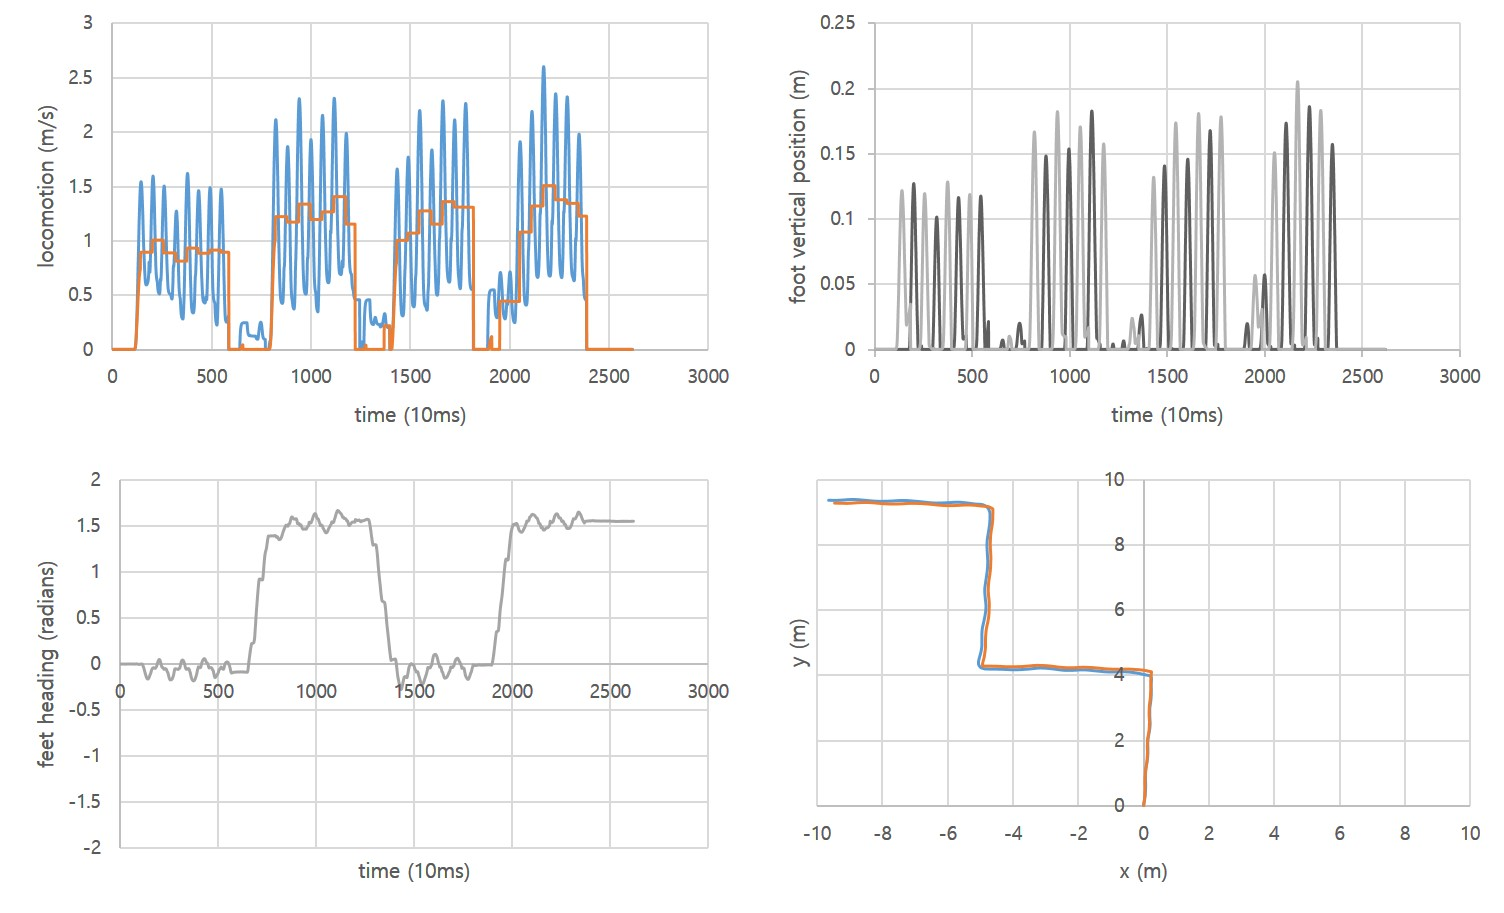
\includegraphics[width=\textwidth,height=\textheight,keepaspectratio]{Figures/session4.jpg}
\decoRule
\caption[WIP session 4]{Locomotion generation for WIP session 4 (natural WIP with rotation). Direct approach is in blue and indirect approach is in orange. Left foot and right foot is in black and grey, respectively.}
\label{fig:wip_session4}
\end{figure}

\begin{figure}[th]
\captionsetup{justification=raggedright,singlelinecheck=false}
\centering
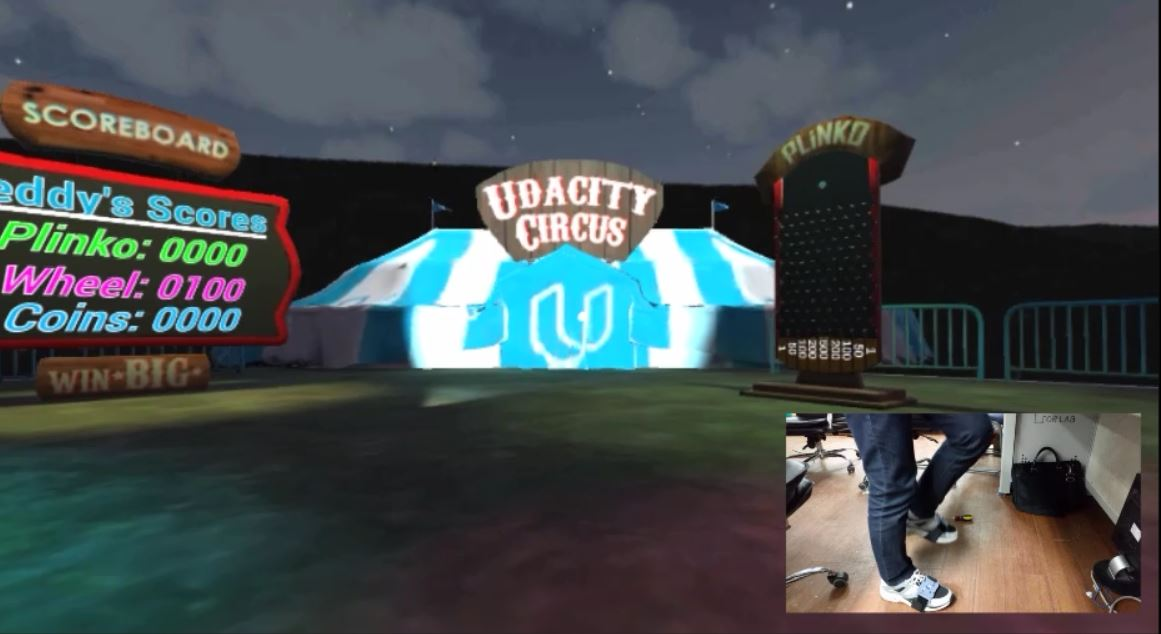
\includegraphics[width=\textwidth,height=\textheight,keepaspectratio]{Figures/demo.jpg}
\decoRule
\caption[Demo]{Demonstration of proposed WIP technique with Unity (sample scene from Udacity)}
\label{fig:demo}
\end{figure}
% Conclusion

\chapter{Conclusion} % Main chapter title

\label{Chapter4} % Change X to a consecutive number; for referencing this chapter elsewhere, use \ref{ChapterX}

%----------------------------------------------------------------------------------------
%	SECTION 1
%----------------------------------------------------------------------------------------

Generating locomotion from WIP motion has been achieved with various setups. LLCM-WIP \citep{Fea08} used magnetic sensors mounted to the knees to track WIP motion and to the chest to determine the heading. GUD-WIP \citep{Wen10} and SAS-WIP \citep{Bru13} both used optical motion capture system with trackers attached to the shins (GUD-WIP) and to the the feet (SAS-WIP), respectively. \cite{Bru17} improved upon SAS-WIP and used a commercial hardware (Microsoft Kinect) instead of an optical motion capture system. Recently there has been attempts such as the VR-STEP \citep{Tre16} to implement the WIP technique with on-board smartphone sensors only. Though it lacks sophistication such as variable locomotion speeds with spatio-temporal WIP parameters achieved in other setups, no custom hardware is required. 
\\\\
The setup proposed in this paper retains the level of sophistication of the most recent research and at the same time reduces the bulk and the cost of additional hardware required. Moreover, unlike some setups in the literature, the inside-out nature of this setup does not require external sensor arrays which allows for a hassle free user experience. For research purposes LPMS-B2 modules costing 300\$ each was used. However, consumer-grade MEMS IMU sensor which is inexpensive and small enough to be integrated in the shoe, is adequate for the setup proposed in this paper. Future studies might focus on developing custom hardware and conducting user surveys to further iron out issues and improve performance metrics.
%\include{Chapters/Chapter2} 
%\include{Chapters/Chapter3}
%\include{Chapters/Chapter4} 
%\include{Chapters/Chapter5} 

%----------------------------------------------------------------------------------------
%	THESIS CONTENT - APPENDICES
%----------------------------------------------------------------------------------------

\appendix % Cue to tell LaTeX that the following "chapters" are Appendices

% Include the appendices of the thesis as separate files from the Appendices folder
% Uncomment the lines as you write the Appendices

%% Appendix A

\chapter{Frequently Asked Questions} % Main appendix title

\label{AppendixA} % For referencing this appendix elsewhere, use \ref{AppendixA}

\section{How do I change the colors of links?}

The color of links can be changed to your liking using:

{\small\verb!\hypersetup{urlcolor=red}!}, or

{\small\verb!\hypersetup{citecolor=green}!}, or

{\small\verb!\hypersetup{allcolor=blue}!}.

\noindent If you want to completely hide the links, you can use:

{\small\verb!\hypersetup{allcolors=.}!}, or even better: 

{\small\verb!\hypersetup{hidelinks}!}.

\noindent If you want to have obvious links in the PDF but not the printed text, use:

{\small\verb!\hypersetup{colorlinks=false}!}.

%\include{Appendices/AppendixB}
%\include{Appendices/AppendixC}

%----------------------------------------------------------------------------------------
%	BIBLIOGRAPHY
%----------------------------------------------------------------------------------------

\printbibliography[heading=bibintoc]

%----------------------------------------------------------------------------------------

\end{document}  
